\documentclass[11pt]{article}

\usepackage[english]{babel}
\usepackage[utf8]{inputenc}
\usepackage[T1]{fontenc}
\usepackage{lmodern}
\usepackage[margin=2.1cm, headheight=14pt]{geometry}
\usepackage{amsmath, amssymb, mathtools}
\usepackage{graphicx}
\usepackage{booktabs}
\usepackage{enumitem}
\usepackage{fancyhdr}
\usepackage{xcolor}
\usepackage[most]{tcolorbox}
\usepackage{tikz}
\usetikzlibrary{arrows.meta}
\usepackage[colorlinks=true, allcolors=blue!55!black]{hyperref}

\graphicspath{{figures/}}
\setlength{\emergencystretch}{3em}
\setlength{\parindent}{0pt}
\setlength{\parskip}{3pt}
\numberwithin{equation}{section}
\allowdisplaybreaks
\setlist{itemsep=1pt, topsep=2pt, leftmargin=*}

\definecolor{srccol}{RGB}{25,85,165}
\definecolor{owncol}{RGB}{190,80,0}
\definecolor{whycol}{RGB}{105,105,105}

\newcommand{\dd}{\mathrm{d}}
\newcommand{\erf}{\operatorname{erf}}
\newcommand{\erfc}{\operatorname{erfc}}
\newcommand{\lth}{\lambda_{\mathrm{th}}}
\newcommand{\Cq}{C_v^{\mathrm{q}}}
\newcommand{\Ccl}{C_v^{\mathrm{cl}}}
\newcommand{\kB}{k_B}
\newcommand{\Hpt}{H_{\mathrm{PT}}}
\newcommand{\Ad}{A^{\dagger}}
\newcommand{\hs}{\tfrac{\hbar}{\sqrt{2m}}}
\newcommand{\Eu}{\hbar^2\alpha^2/2m}
\newcommand{\tL}{\tanh(\alpha L/2)}
\newcommand{\why}[1]{\text{\footnotesize\color{whycol}#1}}
\newcommand{\src}[1]{\par\noindent{\footnotesize\textcolor{srccol}{\textsf{\textbf{Source.}} #1}}\par}
\newcommand{\own}[1]{\par\noindent{\footnotesize\textcolor{owncol}{\textsf{\textbf{Own step.}} #1}}\par}
\newcommand{\fact}[2]{\par\medskip\noindent\textbf{#1\enspace #2.}\enspace}
\newcommand{\chk}[1]{{\footnotesize\textsf{(#1)}}}

\newtcolorbox{result}{colback=gray!7, colframe=black!65, boxrule=0.6pt, arc=2pt,
  left=2mm, right=2mm, top=0.5mm, bottom=0.5mm}
\newtcolorbox{intuition}{colback=srccol!3, colframe=srccol!55, boxrule=0.5pt, arc=2pt,
  left=2mm, right=2mm, top=1mm, bottom=1mm, breakable, title={Intuition},
  fonttitle=\small\bfseries, coltitle=black, colbacktitle=srccol!10}
\newtcolorbox{guide}[1]{colback=gray!4, colframe=black!55, boxrule=0.5pt, arc=2pt,
  left=2mm, right=2mm, top=1mm, bottom=1mm, breakable, title={#1},
  fonttitle=\small\bfseries, coltitle=black, colbacktitle=gray!14}

\pagestyle{fancy}
\fancyhf{}
\lhead{\small 00540367: Research Project 1}
\rhead{\small Technion - IIT}
\lfoot{\small Spring 2026 | Semester 6}
\rfoot{\small Page \thepage}
\renewcommand{\headrulewidth}{0.4pt}
\renewcommand{\footrulewidth}{0.4pt}

\begin{document}

\begin{center}
{\LARGE\bfseries P\"oschl--Teller Well in a Box}\\[2mm]
{\large Every step of the derivation of $\Cq$ and $\Ccl$, from Calculus~1--2 and linear algebra}\\[2mm]
{\small Nadav Jean \quad$\cdot$\quad 28.10.2026 \quad$\cdot$\quad companion to \texttt{PT\_Box\_Summary.pdf} and \texttt{PT\_Box\_Derivation.pdf}}
\end{center}
\thispagestyle{fancy}

\begin{guide}{How to read this}
\textbf{Prerequisites.} Calculus 1--2 and linear algebra. Every other tool is built in \S\ref{sec:math} (mathematics, facts F1--F15) and \S\ref{sec:phys} (physics, P1--P5); later steps cite these labels.

\textbf{Two routes to the energy levels.} The main text solves the Schr\"odinger equation by factorization (``SUSY'', \S\ref{sec:levels}.1--\ref{sec:walls}). \S\ref{sec:legendre} derives the same solutions with associated Legendre functions, and \S\ref{sec:routes} compares the two and recommends one.

\textbf{Labels under a step.}
\textcolor{srccol}{\textsf{\textbf{Source.}}} The statement (or its result) is in that source, on the page given. Every page was checked against the copy listed in the References.
\textcolor{owncol}{\textsf{\textbf{Own step.}}} Constructed for this project by Claude, the AI assistant that wrote the earlier derivation. ``No reference found'' means no published source was found for it. ``(standard)'' means Claude's write-up of a textbook argument; the result itself is cited where a page-checked source exists.

\textbf{Checks.} (C$n$) is block $n$ of \texttt{check\_explained.py} in this folder. It recomputes every number quoted here in about 1~min; its output is in \texttt{results/check\_explained.log}.

\textbf{Units.} Temperatures are given as $\kB T$ in units of $\Eu$, and box sizes as $\alpha L$.

\textbf{Not covered.} Homogeneous strokes and the engine (Derivation \S7).
\end{guide}

\begin{center}
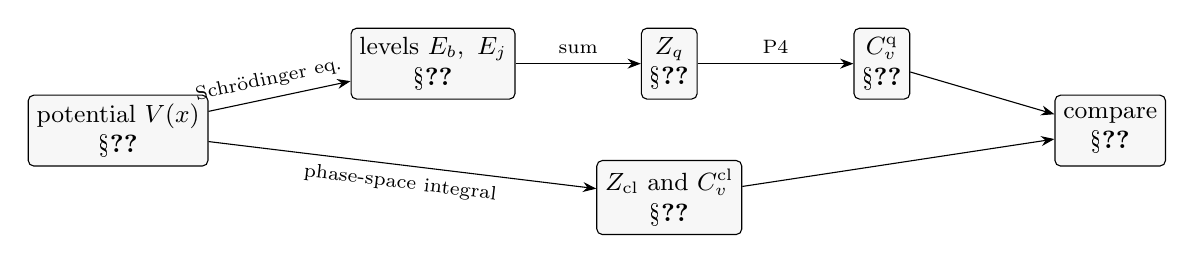
\begin{tikzpicture}[>=Stealth, box/.style={draw, rounded corners=2pt, align=center, font=\small, inner sep=3pt, fill=gray!6, minimum height=9mm}]
\node[box] (V) at (0,0) {potential $V(x)$\\\S\ref{sec:model}};
\node[box] (E) at (4.0,0.85) {levels $E_b,\ E_j$\\\S\ref{sec:levels}};
\node[box] (Zq) at (7.0,0.85) {$Z_q$\\\S\ref{sec:Zq}};
\node[box] (Cq) at (9.7,0.85) {$\Cq$\\\S\ref{sec:Cq}};
\node[box] (Zcl) at (7.0,-0.85) {$Z_{\rm cl}$ and $\Ccl$\\\S\ref{sec:classical}};
\node[box] (cmp) at (12.6,0) {compare\\\S\ref{sec:compare}};
\draw[->] (V) -- node[above, sloped, pos=0.45, font=\scriptsize] {Schr\"odinger eq.} (E);
\draw[->] (E) -- node[above, font=\scriptsize] {sum} (Zq);
\draw[->] (Zq) -- node[above, font=\scriptsize] {P4} (Cq);
\draw[->] (V) -- node[below, sloped, font=\scriptsize] {phase-space integral} (Zcl);
\draw[->] (Cq) -- (cmp);
\draw[->] (Zcl) -- (cmp);
\end{tikzpicture}
\end{center}

\begin{guide}{Assumptions}
\begin{enumerate}[label=\textbf{A\arabic*}, itemsep=0pt]
\item One particle of mass $m$ in one dimension, in equilibrium with a heat bath at temperature $T$ (canonical ensemble), $\beta=1/\kB T$.
\item The P\"oschl--Teller well with $\lambda=2$, Eq.~\eqref{eq:V}, inside hard walls at $x=\pm L/2$.
\item $\alpha L\gg1$. Terms of relative size $e^{-\alpha L}$ are dropped; for $\alpha L\ge100$ these are below $4\times10^{-44}$.
\item $L\gtrsim2\lth$. The sum-to-integral remainder $R$ of \S\ref{sec:Zq} is dropped.
\end{enumerate}
Apart from A3--A4, the closed forms \eqref{eq:Zq}, \eqref{eq:Cq} and \eqref{eq:Ccl} are exact. Both are checked against exact level sums (C11, C13, C14).
\end{guide}

\tableofcontents

% =====================================================================
\section{Mathematical toolkit}
\label{sec:math}

\fact{F1}{Hyperbolic functions}
$\displaystyle\cosh u=\frac{e^{u}+e^{-u}}{2},\quad \sinh u=\frac{e^{u}-e^{-u}}{2},\quad \tanh u=\frac{\sinh u}{\cosh u}.$
\begin{enumerate}[label=(\alph*)]
\item $\cosh^2u-\sinh^2u=1$, hence $1-\tanh^2u=\dfrac{1}{\cosh^2u}$.\quad Proof: $(e^u+e^{-u})^2-(e^u-e^{-u})^2=4$. Divide by 4, then by $\cosh^2u$.
\item $(\cosh u)'=\sinh u$, $(\sinh u)'=\cosh u$, $(\tanh u)'=\dfrac{\cosh^2u-\sinh^2u}{\cosh^2u}=\dfrac{1}{\cosh^2u}$ (quotient rule, then (a)).
\item $\cosh$ is even; $\sinh$ and $\tanh$ are odd (replace $u$ by $-u$ in the definitions).
\item $\sinh2u=2\sinh u\cosh u$ and $\cosh^2u=\frac12(1+\cosh2u)$ (expand both sides).
\item For $u>0$: $0<1-\tanh u=\dfrac{2}{e^{2u}+1}<2e^{-2u}$ and $0<\dfrac{1}{\cosh^2u}<4e^{-2u}$. So as $u\to\pm\infty$, $\tanh u\to\pm1$ and $1/\cosh^2u\to0$, exponentially fast.\quad Proof: $1-\tanh u=\frac{\cosh u-\sinh u}{\cosh u}=\frac{e^{-u}}{\cosh u}$, and $\cosh u>\frac12e^{u}$.
\item $\cosh u-\tanh u\,\sinh u=\dfrac{1}{\cosh u}$ (by (a)), and $\tanh u\,\cosh u=\sinh u$.
\end{enumerate}
\src{[DLMF] 4.28.1, 4.28.2, 4.28.4 (definitions); 4.35.11--12 (a); 4.34.1--3 (b); 4.35.23--25 (c); 4.35.26--27 (d).}
\own{(standard) (e) and (f) follow from the definitions; no source checked.}

\fact{F2}{arctan and tan}
$\arctan:\mathbb R\to(-\frac\pi2,\frac\pi2)$ is the inverse of $\tan$ on $(-\frac\pi2,\frac\pi2)$.
\begin{enumerate}[label=(\alph*)]
\item $\arctan(-u)=-\arctan u$, and $(\arctan u)'=\dfrac{1}{1+u^2}$. Hence, for $c>0$ (substitute $u=cv$): $\displaystyle\int_0^\infty\frac{\dd u}{u^2+c^2}=\frac1c\big[\arctan v\big]_0^\infty=\frac{\pi}{2c}$.
\item For $u>0$: $\arctan\frac1u=\frac\pi2-\arctan u$.\quad Proof: by (a), the sum $\arctan\frac1u+\arctan u$ has derivative $-\frac{1/u^2}{1+1/u^2}+\frac{1}{1+u^2}=0$, so it is constant. At $u=1$ it equals $\frac\pi4+\frac\pi4$.
\item $\tan$ has period $\pi$ and is one-to-one on each period: $\tan\varphi_1=\tan\varphi_2\iff\varphi_1=\varphi_2+n\pi$, $n\in\mathbb Z$.
\item $\tan(\varphi+\frac\pi2)=-\dfrac{1}{\tan\varphi}$, because $\sin(\varphi+\frac\pi2)=\cos\varphi$ and $\cos(\varphi+\frac\pi2)=-\sin\varphi$.
\end{enumerate}
\src{[DLMF] 4.23.12 and 4.24.9 (a); 4.23.9 with 4.23.18 (b); 4.14.10 (c).}

\fact{F3}{Functions as vectors, operators as linear maps}
The functions on an interval form a vector space. The maps $f\mapsto f'$, $f\mapsto W(x)f$ and $f\mapsto-\frac{\hbar^2}{2m}f''+V(x)f$ are linear; physicists call them \emph{operators}. A product of operators is their composition, $(ST)f=S(Tf)$. Composition is associative, but in general $ST\neq TS$, exactly as for matrices. The equation $H\psi=E\psi$ with $\psi\neq0$ is an eigenvalue equation, the analogue of $Au=\lambda u$.

\emph{Lemma (intertwining).} If $ST=TR$ and $R\varphi=E\varphi$, then $S(T\varphi)=E\,(T\varphi)$.\quad
Proof: $S(T\varphi)=(ST)\varphi=(TR)\varphi=T(R\varphi)=T(E\varphi)=E\,T\varphi$. $\square$ So, when $T\varphi\neq0$, it is an eigenvector of $S$ with the same eigenvalue. This is the same mechanism by which similar matrices share eigenvalues.
\src{$H\psi=E\psi$ as the analogue of $Au=\lambda u$: [Tong-QM, p.~68].}
\own{(standard) The lemma.}

\fact{F4}{All solutions of the three free equations}
On an interval containing $0$, with $k>0$ and $\kappa>0$:
\begin{align*}
&\text{(a) }\varphi''=-k^2\varphi\iff\varphi=C_1\cos kx+C_2\sin kx;\qquad
\text{(b) }\varphi''=0\iff\varphi=C_1+C_2x;\\
&\text{(c) }\varphi''=\kappa^2\varphi\iff\varphi=C_1\cosh\kappa x+C_2\sinh\kappa x.
\end{align*}
Proof. ``$\Leftarrow$'': differentiate (F1b). ``$\Rightarrow$'':
(a) $u\equiv\varphi-\varphi(0)\cos kx-\frac{\varphi'(0)}{k}\sin kx$ solves $u''=-k^2u$ with $u(0)=u'(0)=0$. Then $\frac{\dd}{\dd x}\big(u'^2+k^2u^2\big)=2u'(u''+k^2u)=0$. So $u'^2+k^2u^2$ is constant, equal to its value $0$ at $x=0$; hence $u\equiv0$.
(b) $\varphi'$ is constant.
(c) $u\equiv\varphi-\varphi(0)\cosh\kappa x-\frac{\varphi'(0)}{\kappa}\sinh\kappa x$ solves $u''=\kappa^2u$ with $u(0)=u'(0)=0$. Let $v\equiv u'-\kappa u$. Then $v'=\kappa^2u-\kappa u'=-\kappa v$, so $(e^{\kappa x}v)'=0$ and $v\equiv v(0)=0$. Then $(e^{-\kappa x}u)'=e^{-\kappa x}v=0$, so $u\equiv u(0)=0$. $\square$

Each solution space is two-dimensional, spanned by one even and one odd function.
\own{(standard) No page-checked reference. The ``conserved combination'' trick is the Wronskian argument of [Tong-QM, pp.~49--50].}

\fact{F5}{Integrating factor}
If $y'+p(x)\,y=q(x)$ and $P'=p$, then $(e^{P}y)'=e^{P}(y'+py)=e^{P}q$ (product rule).
\own{(standard) No page-checked reference.}

\fact{F6}{Gaussian integral}
For $s>0$: $\displaystyle\int_0^\infty e^{-su^2}\dd u=\frac12\sqrt{\frac\pi s}$ and $\displaystyle\int_{-\infty}^{\infty}e^{-su^2}\dd u=\sqrt{\frac\pi s}$.

Proof (Calc~2, polar coordinates). Let $g\equiv\int_0^\infty e^{-u^2}\dd u$. Then
$g^2=\int_0^\infty\!\!\int_0^\infty e^{-(u^2+v^2)}\dd u\,\dd v=\int_0^{\pi/2}\!\!\int_0^\infty e^{-r^2}r\,\dd r\,\dd\phi=\frac\pi2\cdot\frac12$, so $g=\frac{\sqrt\pi}{2}$. Then substitute $u\to\sqrt s\,u$.
\src{Result: [Tong-SP, p.~35].}
\own{(standard) The proof.}

\fact{F7}{Error function}
$\displaystyle\erf z=\frac{2}{\sqrt\pi}\int_0^ze^{-t^2}\dd t,\qquad \erfc z=1-\erf z=\frac{2}{\sqrt\pi}\int_z^\infty e^{-t^2}\dd t.$
\begin{enumerate}[label=(\alph*)]
\item $\erf0=0$, $\erf(\infty)=1$ (by F6), and $\erf(-z)=-\erf z$.
\item $(\erf z)'=\frac{2}{\sqrt\pi}e^{-z^2}$ (fundamental theorem of calculus). With the chain rule,
$\dfrac{\dd}{\dd a}\erf\sqrt{a/2}=\dfrac{2}{\sqrt\pi}e^{-a/2}\cdot\dfrac{1}{2\sqrt{2a}}=\dfrac{e^{-a/2}}{\sqrt{2\pi a}}$ and $\dfrac{\dd}{\dd a}\erf\sqrt a=\dfrac{e^{-a}}{\sqrt{\pi a}}$.
\item Small $z$: $\erf z=\frac{2}{\sqrt\pi}\big(z-\frac{z^3}{3}+\dots\big)$. Exactly, $e^{z^2}\erf z=\dfrac{2}{\sqrt\pi}\displaystyle\sum_{n\ge0}\frac{2^nz^{2n+1}}{(2n+1)!!}$, where $(2n+1)!!\equiv1\cdot3\cdot5\cdots(2n+1)$.
\item Large $z$: $\erfc z=\dfrac{e^{-z^2}}{\sqrt\pi\,z}\Big(1-\dfrac{1}{2z^2}+\dots\Big)$.
\end{enumerate}
\src{[DLMF] 7.2.1--2 (definitions), 7.4.1 (odd), 7.6.1--2 (c), 7.12.1 (d).}

\fact{F8}{Differentiating under the integral sign}
$\frac{\dd}{\dd s}\int f(s,u)\,\dd u=\int\frac{\partial f}{\partial s}\,\dd u$ holds when $f$ and $\partial f/\partial s$ are continuous on a finite interval. On an infinite interval it needs, in addition, that $\int\partial_sf\,\dd u$ converges uniformly, for example $|\partial_sf|\le g(u)$ with $\int g\,\dd u<\infty$. In every use below, the integrand and its $s$-derivative are either continuous on a finite interval or bounded by $(1+u^2)e^{-s_0u^2}$ for $s\ge s_0>0$.
\src{[DLMF] 1.5.22 (finite interval, with the conditions above) and 1.5.23--24 (infinite interval).}

\fact{F9}{Integrating a series term by term}
$\int_a^b\sum_nf_n=\sum_n\int_a^bf_n$ if the series converges uniformly on $[a,b]$. An example used below: $\sum_{\ell\ge1}\frac{a^\ell v^{\ell-1}}{\ell!}$ on $0\le v\le1$. Its terms are bounded by $\frac{a^\ell}{\ell!}$, and $\sum_\ell\frac{a^\ell}{\ell!}<\infty$ (Weierstrass test).
\src{[DLMF] 1.9.68. (Weierstrass test: standard; no page-checked reference.)}

\fact{F10}{From a sum to an integral (Euler--Maclaurin, even functions)}
Let $F$ be smooth and even on $\mathbb R$ ($F(-y)=F(y)$), with $F$ and all its derivatives integrable and tending to $0$ as $y\to\infty$. Then
\begin{equation}
\sum_{j=1}^{\infty}F(j)=\int_0^\infty F(y)\,\dd y-\frac12F(0)+R,\qquad
|R|\le\frac{1}{12}\int_0^\infty|F''|\,\dd y,\quad
|R|\le\frac{4}{(2\pi)^{2m}}\int_0^\infty|F^{(2m)}|\,\dd y\ (m\ge1).
\label{eq:EM}
\end{equation}
\emph{Step 1.} On $[j,j+1]$ let $P_1(y)=y-j-\frac12$, so $P_1'=1$, $P_1(j)=-\frac12$, $P_1(j+1)=\frac12$. Integrate by parts:
\[
\int_j^{j+1}P_1F'\,\dd y=\big[P_1F\big]_j^{j+1}-\int_j^{j+1}F\,\dd y=\frac{F(j)+F(j+1)}{2}-\int_j^{j+1}F\,\dd y .
\]
Sum over $j=0,1,2,\dots$, using $\sum_{j\ge0}\frac{F(j)+F(j+1)}{2}=\frac{F(0)}{2}+\sum_{j\ge1}F(j)$. The result is \eqref{eq:EM} with $R=\int_0^\infty P_1F'\,\dd y$, where $P_1$ is the sawtooth $y-\lfloor y\rfloor-\frac12$.

\emph{Step 2.} Let $P_2(y)\equiv\frac12\big(s^2-s+\frac16\big)$ with $s=y-\lfloor y\rfloor$. It is continuous, has period 1, satisfies $P_2'=P_1$, and $|P_2|\le\frac1{12}$. Integrating by parts again,
$R=\big[P_2F'\big]_0^\infty-\int_0^\infty P_2F''\,\dd y=-\int_0^\infty P_2F''\,\dd y$, because $F'(0)=0$ ($F$ even, so $F'$ is odd). Hence $|R|\le\frac1{12}\int|F''|$.

\emph{Step 3.} Repeating this, every boundary term at $y=0$ contains either an odd derivative $F^{(2i-1)}(0)=0$ or a factor $P_{2i+1}(0)=0$. The result is $R=-\int_0^\infty P_{2m}F^{(2m)}\,\dd y$ with $\max|P_{2m}|=|B_{2m}|/(2m)!<4/(2\pi)^{2m}$, where $B_{2m}$ are the Bernoulli numbers. $\square$

\emph{Example, exact.} For $F(y)=e^{-\omega y^2}$ ($\omega>0$), $\sum_{n=-\infty}^{\infty}e^{-\omega n^2}=\sqrt{\pi/\omega}\,\big(1+2\sum_{\ell\ge1}e^{-\pi^2\ell^2/\omega}\big)$. With $\sum_{j\ge1}=\frac12\big(\sum_{n=-\infty}^\infty-1\big)$ and F6, this gives
\begin{equation}
R=\sqrt{\frac\pi\omega}\,\sum_{\ell\ge1}e^{-\pi^2\ell^2/\omega}.
\label{eq:Rgauss}
\end{equation}
So $R$ is tiny once $F$ is wide compared with the spacing 1 ($\omega\ll1$) \chk{C9a}.
\src{General formula: [DLMF] 2.10.1. $P_n=\widetilde B_n/n!$ (periodic Bernoulli functions): [DLMF] 24.2.11--12. Bounds: [DLMF] 24.9.1, 24.9.8--9 \chk{C9c}. The Gaussian sum: [DLMF] 1.8.16 with $x=0$.}
\own{(standard) Steps 1--2 and the specialisation to even $F$.}

\fact{F11}{A Gaussian--Lorentzian integral}
For $s>0$ and $c>0$:
\begin{equation}
\mathcal F(s)\equiv\int_0^\infty\frac{e^{-su^2}}{u^2+c^2}\,\dd u=\frac{\pi}{2c}\,e^{sc^2}\erfc\!\big(c\sqrt s\big).
\label{eq:GL}
\end{equation}
Proof:
\begin{align*}
\mathcal F'(s)&=-\int_0^\infty\frac{u^2\,e^{-su^2}}{u^2+c^2}\,\dd u &&\why{F8}\\
\mathcal F'-c^2\mathcal F&=-\int_0^\infty\frac{(u^2+c^2)\,e^{-su^2}}{u^2+c^2}\,\dd u=-\frac12\sqrt{\frac\pi s} &&\why{F6}\\
\big(e^{-c^2s}\mathcal F\big)'&=-\frac12\sqrt{\frac\pi s}\;e^{-c^2s} &&\why{F5 with $p=-c^2$}\\
e^{-c^2s}\mathcal F(s)&=\frac12\int_s^\infty\sqrt{\frac\pi\sigma}\;e^{-c^2\sigma}\dd\sigma &&\why{integrate from $s$ to $\infty$; $e^{-c^2S}\mathcal F(S)\to0$ since $\mathcal F\le\frac{\pi}{2c}$ (F2a)}\\
&=\frac{\sqrt\pi}{c}\int_{c\sqrt s}^\infty e^{-v^2}\dd v=\frac{\pi}{2c}\erfc\big(c\sqrt s\big) &&\why{$\sigma=v^2/c^2$, $\dd\sigma=2v\,\dd v/c^2$; F7}
\end{align*}
Multiply by $e^{c^2s}$. As a check, $s\to0$ gives $\frac{\pi}{2c}$, as F2a requires \chk{C10}.
\src{Result: [DLMF] 7.7.1 (put $u=ct$, $z=c\sqrt s$).}
\own{The proof. No reference found for this route.}

\fact{F12}{A polynomial integral}
For $n=0,1,2,\dots$: $\displaystyle W_n\equiv\int_{-1}^{1}(1-t^2)^n\,\dd t=\frac{2^{n+1}\,n!}{(2n+1)!!}$.

Proof: $W_0=2$. For $n\ge1$, integrate by parts with $\dd v=\dd t$:
$W_n=\big[t(1-t^2)^n\big]_{-1}^{1}+2n\int_{-1}^{1}t^2(1-t^2)^{n-1}\dd t=2n\int_{-1}^{1}\big[1-(1-t^2)\big](1-t^2)^{n-1}\dd t=2n\,(W_{n-1}-W_n)$.
So $W_n=\frac{2n}{2n+1}W_{n-1}=2\cdot\frac{2\cdot4\cdots2n}{3\cdot5\cdots(2n+1)}=\frac{2\cdot2^n\,n!}{(2n+1)!!}$. $\square$ \chk{C10}
\src{Equivalent to Euler's Beta integral, [DLMF] 5.12.1 (with 5.4.6 and 5.5.1).}
\own{(standard) The recursion.}

\emph{F13--F15 are used only in the second route of \S\ref{sec:legendre}.}

\fact{F13}{Complex numbers}
$i^2=-1$ and $e^{i\theta}=\cos\theta+i\sin\theta$, so $e^{\pm ikx}=\cos kx\pm i\sin kx$. If $w=u+iv$ (with $u,v$ real) solves a linear ODE whose coefficients are real, then $u$ and $v$ each solve it: take the real and imaginary parts of the equation.
\src{$\cos z\pm i\sin z=e^{\pm iz}$: [DLMF] 4.14.3.}
\own{(standard) The real/imaginary-part remark.}

\fact{F14}{Gamma function}
$\Gamma(z)=\int_0^\infty e^{-t}t^{z-1}\dd t$ for $\mathrm{Re}\,z>0$. Integration by parts gives $\Gamma(z+1)=\big[-e^{-t}t^z\big]_0^\infty+z\int_0^\infty e^{-t}t^{z-1}\dd t=z\,\Gamma(z)$; with $\Gamma(1)=1$ this gives $\Gamma(n+1)=n!$. $\Gamma$ extends to all complex $z$ except $z=0,-1,-2,\dots$, where it has poles. It has no zeros, so $1/\Gamma(z)$ is finite everywhere and vanishes exactly at $z=0,-1,-2,\dots$
\src{[DLMF] 5.2.1 (definition), 5.5.1 ($\Gamma(z+1)=z\Gamma(z)$); poles, no zeros and $1/\Gamma$: the text after 5.2.1 in \S5.2(i).}
\own{(standard) The integration by parts.}

\fact{F15}{Hypergeometric series}
With the rising factorial $(a)_0=1$, $(a)_s=a(a+1)\cdots(a+s-1)$,
$\displaystyle F(a,b;c;z)=\sum_{s\ge0}\frac{(a)_s(b)_s}{(c)_s\,s!}\,z^s=1+\frac{ab}{c}z+\frac{a(a+1)b(b+1)}{c(c+1)\,2!}z^2+\dots$
If $b=-m$ with $m=0,1,2,\dots$, then $(b)_s=0$ for $s>m$ and the series stops: $F$ is a polynomial of degree $m$. For $m=1$: $F(a,-1;c;z)=1-\frac{a}{c}\,z$.
\src{[DLMF] 5.2.4--5 (rising factorial), 15.2.1 (series), 15.2.4 (terminating case).}

% =====================================================================
\section{Physics toolkit}
\label{sec:phys}

\fact{P1}{Quantum energy levels}
$H=-\frac{\hbar^2}{2m}\frac{\dd^2}{\dd x^2}+V(x)$ is a linear map (F3). The allowed energies are its eigenvalues: the values of $E$ for which $H\psi=E\psi$ has a solution $\psi\not\equiv0$ obeying the boundary conditions. $\psi$ and $C\psi$ ($C\neq0$) are the same state. At a hard wall $V=+\infty$, which forces $\psi=0$ there; $\psi$ is continuous, so $\psi(\pm L/2)=0$.
\src{[Tong-QM, p.~9, Eq.~(1.1); p.~10, Eq.~(1.2); p.~68]. Hard walls: [Tong-QM, pp.~24--25].}

\emph{Example: the empty box} ($V=0$ for $|x|<L/2$), solved with F4. Section~\ref{sec:levels} repeats exactly these steps for the well.
\begin{itemize}
\item $E=\frac{\hbar^2k^2}{2m}>0$. Then $\psi=C_1\cos kx+C_2\sin kx$, and $\psi(\frac L2)\pm\psi(-\frac L2)=0$ means $C_1\cos\frac{kL}{2}=0$ and $C_2\sin\frac{kL}{2}=0$. A nonzero $\psi$ needs $\cos\frac{kL}2=0$ or $\sin\frac{kL}2=0$, i.e.\ $kL=n\pi$ with $n=1,2,\dots$
\item $E=0$: $C_1+C_2x$ vanishes at $\pm\frac L2$ only if $C_1=C_2=0$. $E<0$: $C_1\cosh\frac{\kappa L}2=0=C_2\sinh\frac{\kappa L}2$ forces $C_1=C_2=0$.
\end{itemize}
\begin{equation}
E_n=n^2E_1,\qquad E_1=\frac{\pi^2\hbar^2}{2mL^2},\qquad n=1,2,3,\dots
\label{eq:boxlevels}
\end{equation}
\src{[Tong-QM, p.~25, Eq.~(2.10)] (box $0<x<L$, same levels).}
\own{(standard) The derivation via F4.}

\fact{P2}{Parity}
If $V(-x)=V(x)$ and $\psi(x)$ solves $H\psi=E\psi$, then so does $\psi(-x)$ (chain rule). The solutions can therefore be chosen even or odd. If $\psi=c_e\psi_e+c_o\psi_o$ with $\psi_e$ even and $\psi_o$ odd, then $\psi(\pm\frac L2)=c_e\psi_e(\frac L2)\pm c_o\psi_o(\frac L2)$. Adding and subtracting,
\begin{equation}
\psi(\pm L/2)=0\iff c_e\,\psi_e(L/2)=0\ \text{ and }\ c_o\,\psi_o(L/2)=0 .
\label{eq:parityBC}
\end{equation}
\src{Parity: [Tong-Topics, p.~196].}
\own{(standard) Eq.~\eqref{eq:parityBC}.}

\fact{P3}{Canonical ensemble}
In equilibrium with a bath at temperature $T$, level $n$ is occupied with probability
$p_n=e^{-\beta E_n}/Z$, where $Z=\sum_ne^{-\beta E_n}$ and $\beta=1/\kB T$.
\src{[Tong-SP, p.~18, Eqs.~(1.19)--(1.22)].}

\fact{P4}{Heat capacity from $Z$}
\begin{equation}
U\equiv\langle E\rangle=-\frac{\partial\ln Z}{\partial\beta},\quad
\frac{\partial^2\ln Z}{\partial\beta^2}=\langle E^2\rangle-\langle E\rangle^2\equiv\mathrm{Var}(E),\quad
C_v\equiv\frac{\dd U}{\dd T}=\kB\beta^2\,\frac{\partial^2\ln Z}{\partial\beta^2}=\kB\beta^2\,\mathrm{Var}(E).
\label{eq:Cv}
\end{equation}
Proof: $\partial_\beta Z=-\sum_nE_ne^{-\beta E_n}$, so $-\partial_\beta\ln Z=\sum_nE_np_n$. Next $\partial_\beta^2Z=\sum_nE_n^2e^{-\beta E_n}$, so $\partial_\beta^2\ln Z=\frac{\partial_\beta^2Z}{Z}-\big(\frac{\partial_\beta Z}{Z}\big)^2=\langle E^2\rangle-\langle E\rangle^2$. Finally $\frac{\dd\beta}{\dd T}=-\frac{1}{\kB T^2}=-\kB\beta^2$ and $\frac{\dd U}{\dd T}=\frac{\dd U}{\dd\beta}\frac{\dd\beta}{\dd T}$. $\square$
\src{[Tong-SP, p.~20, Eqs.~(1.25)--(1.27)].}
Consequences:
\begin{enumerate}[label=(\alph*)]
\item $C_v\ge0$.
\item Multiplying $Z$ by a constant, or shifting every $E_n$ by the same constant, leaves $C_v$ unchanged: $\ln Z$ changes by a constant or by a term linear in $\beta$.
\item If $Z=Z_1Z_2$, then $C_v=C_1+C_2$.
\item If $a=D\beta$ with $D>0$ constant, then $\beta\partial_\beta=a\partial_a$ and $\beta^2\partial_\beta^2=a^2\partial_a^2$, so
\begin{equation}
\frac{C_v}{\kB}=a^2\,\frac{\dd^2\ln Z}{\dd a^2}=a^2\left[\frac{Z''}{Z}-\left(\frac{Z'}{Z}\right)^2\right],\qquad{}'=\frac{\dd}{\dd a}.
\label{eq:Cva}
\end{equation}
\item \emph{Sign rule.} If $\ln Z_1-\ln Z_2=-C\beta^p$ with $C>0$, then $(C_1-C_2)/\kB=-C\,p(p-1)\,\beta^p$, which is positive iff $0<p<1$ \chk{C18a}.
\item \emph{Two-level (Schottky) model.} Take one ground state and $g$ states at height $\Delta$, so $Z=1+ge^{-\beta\Delta}$. Let $P=\frac{ge^{-\beta\Delta}}{1+ge^{-\beta\Delta}}$, the probability of being up. Then $-\partial_\beta\ln Z=\Delta P$ and $\partial_\beta P=-\Delta P(1-P)$, so $C_v/\kB=(\beta\Delta)^2P(1-P)$. The peak is about $(\beta\Delta)^2/4$, at $P=\frac12$, i.e.\ $ge^{-\beta\Delta}=1$. At low $T$, $C_v\approx\kB(\beta\Delta)^2g\,e^{-\beta\Delta}$, which goes to $0$ exponentially because of the gap $\Delta$.
\end{enumerate}
\src{(f): the two-state system and its exponential fall-off due to the gap, [Tong-SP, p.~13, Eq.~(1.14)].}
\own{(a)--(e), and (f) with $g$ upper states.}

\fact{P5}{Classical particle}
\begin{equation}
Z_{\rm cl}=\frac{1}{2\pi\hbar}\int\dd x\int_{-\infty}^{\infty}\dd p\;e^{-\beta\left(\frac{p^2}{2m}+V(x)\right)}=\frac{1}{\lth}\int e^{-\beta V(x)}\,\dd x,\qquad \lth\equiv\sqrt{\frac{2\pi\hbar^2\beta}{m}}.
\label{eq:Zclgen}
\end{equation}
The second form uses $\int e^{-\beta p^2/2m}\dd p=\sqrt{2\pi m/\beta}$ (F6 with $s=\beta/2m$) and $\frac{1}{2\pi\hbar}\sqrt{\frac{2\pi m}{\beta}}=\sqrt{\frac{m}{2\pi\hbar^2\beta}}=\frac{1}{\lth}$. The factor $\frac{1}{2\pi\hbar}$ makes $Z$ dimensionless and makes it agree with the quantum $Z$ at high $T$; by P4(b) it does not affect $C_v$. $\lth$ is the thermal de Broglie wavelength, and $L/\lth$ counts how many of them fit in a length $L$.
\src{[Tong-SP, p.~32, Eq.~(2.1) and the $1/h$ factor; pp.~33--34, the one-dimensional form derived from the quantum $Z$; p.~35, Eqs.~(2.5)--(2.6)].}

Split $Z_{\rm cl}=\big[\sqrt{m/2\pi\hbar^2}\;\beta^{-1/2}\big]\times\int e^{-\beta V}\dd x$ and use P4(c). The first factor gives $\beta^2\partial_\beta^2(-\frac12\ln\beta)=\frac12$. The second factor is P4 with ``levels'' $V(x)$ labelled by $x$. Together,
\begin{equation}
\Ccl=\frac{\kB}{2}+\kB\beta^2\,\mathrm{Var}_x(V),\qquad\text{averaged over } P(x)=\frac{e^{-\beta V(x)}}{\int e^{-\beta V}\,\dd x}.
\label{eq:Cclsplit}
\end{equation}
\emph{Equipartition}: each quadratic term in $H$ contributes $\frac12\kB T$ to $U$. A classical harmonic oscillator therefore has $U=\kB T$ and $C_v=\kB$.
\src{Equipartition: [Tong-SP, p.~37]. Oscillator: [Tong-SP, p.~47, Eq.~(2.20)] and [LGK, p.~95].}
\own{(standard) Eq.~\eqref{eq:Cclsplit}.}

% =====================================================================
\section{The model}
\label{sec:model}
\begin{equation}
V(x)=\begin{cases}-\dfrac{\hbar^2}{2m}\,\alpha^2\,\dfrac{\lambda(\lambda-1)}{\cosh^2(\alpha x)}, & |x|<L/2,\\[8pt] +\infty, & |x|\ge L/2.\end{cases}
\label{eq:Vgen}
\end{equation}
\src{Inside the box, the ``modified P\"oschl--Teller'' row of [DJdC, p.~021013-9, Table~I], where $q$ stands for our $x$. The table takes it from Fl\"ugge, which is not checked here (no free copy found).}
For $\lambda=2$, $\lambda(\lambda-1)=2$ and
\begin{equation}
V(x)=-\frac{\hbar^2\alpha^2}{m}\;\frac{1}{\cosh^2(\alpha x)}\qquad(|x|<L/2).
\label{eq:V}
\end{equation}
The depth is $\hbar^2\alpha^2/m$, at $x=0$. By F1e, $|V(x)|<\frac{4\hbar^2\alpha^2}{m}e^{-2\alpha|x|}$, so the width is about $1/\alpha$ and $|V(\pm L/2)|<\frac{4\hbar^2\alpha^2}{m}e^{-\alpha L}$.

\textbf{Why $\lambda=2$.} The well $-n(n+1)\,\mathrm{sech}^2x$ ``holds $n$ bound states'' and is reflectionless [CKS, p.~77, Eq.~(312); pp.~41--42]. CKS write $\mathrm{sech}=1/\cosh$ and use units $\hbar=2m=\alpha=1$. Since $n(n+1)=\lambda(\lambda-1)=2$ gives $n=1$, $\lambda=2$ is the smallest integer $\lambda$ that binds, and it binds exactly one state; \S\ref{sec:levels} proves this inside the box.

\textbf{Only two dimensionless numbers.} The inputs are $\hbar$, $m$, $\alpha$ (an inverse length), $L$ and $\kB T$. From $\hbar$, $m$ and $\alpha$ one can form exactly one length, $1/\alpha$ (the well width), and one energy, $\hbar^2\alpha^2/m$ (the depth). A dimensionless output such as $C_v/\kB$ can therefore depend only on
\begin{equation}
\alpha L\ \ (\text{box length in well widths})\qquad\text{and}\qquad a\equiv\frac{\beta\hbar^2\alpha^2}{m}=\frac{\text{well depth}}{\kB T}.
\label{eq:dimless}
\end{equation}
With $\lth$ from \eqref{eq:Zclgen}, $\lth^2=\frac{2\pi\hbar^2\beta}{m}=\frac{2\pi a}{\alpha^2}$, hence
\begin{equation}
\alpha\lth=\sqrt{2\pi a},\qquad \frac{L}{\lth}=\frac{\alpha L}{\sqrt{2\pi a}},\qquad \frac{\kB T}{\hbar^2\alpha^2/2m}=\frac{2}{a}.
\label{eq:helpers}
\end{equation}
\own{The dimensional argument and Eq.~\eqref{eq:helpers}.}

% =====================================================================
\section{The energy levels}
\label{sec:levels}
Inside the box we must solve
\begin{equation}
\Hpt\psi\equiv-\frac{\hbar^2}{2m}\psi''-\frac{\hbar^2\alpha^2}{m}\frac{1}{\cosh^2(\alpha x)}\,\psi=E\,\psi\quad(|x|<L/2),\qquad \psi(\pm L/2)=0 .
\label{eq:SE}
\end{equation}
The plan has three steps. (i) Factor $\Hpt$. (ii) Map every solution of the free equation to a solution of \eqref{eq:SE}, and show that these are all of its solutions. (iii) Impose $\psi(\pm L/2)=0$. \S\ref{sec:legendre} reaches the same solutions by a second route (associated Legendre functions), and \S\ref{sec:routes} compares the two.

\subsection{Factorization}
Define
\begin{equation}
W(x)\equiv\frac{\hbar\alpha}{\sqrt{2m}}\tanh(\alpha x),\qquad A\equiv\frac{\hbar}{\sqrt{2m}}\frac{\dd}{\dd x}+W,\qquad \Ad\equiv-\frac{\hbar}{\sqrt{2m}}\frac{\dd}{\dd x}+W .
\label{eq:Adef}
\end{equation}
(Here ``$\dagger$'' is only a name.) For any twice-differentiable $f$, by the product rule:
\begin{align}
\Ad Af&=\Big(-\hs\frac{\dd}{\dd x}+W\Big)\Big(\hs f'+Wf\Big)
=-\frac{\hbar^2}{2m}f''-\hs(W'f+Wf')+\hs Wf'+W^2f\nonumber\\
&=-\frac{\hbar^2}{2m}f''+\Big(W^2-\hs W'\Big)f, \label{eq:AdA}\\
A\Ad f&=\hs\Big(-\hs f'+Wf\Big)'+W\Big(-\hs f'+Wf\Big)
=-\frac{\hbar^2}{2m}f''+\Big(W^2+\hs W'\Big)f. \label{eq:AAd}
\end{align}
Now $W^2=\frac{\hbar^2\alpha^2}{2m}\tanh^2(\alpha x)$ and $\hs W'=\frac{\hbar^2\alpha^2}{2m}\frac{1}{\cosh^2(\alpha x)}$ (F1b). With $\tanh^2=1-1/\cosh^2$ (F1a):
\[
W^2-\hs W'=\frac{\hbar^2\alpha^2}{2m}\Big(1-\frac{2}{\cosh^2(\alpha x)}\Big)=\frac{\hbar^2\alpha^2}{2m}-\frac{\hbar^2\alpha^2}{m}\frac{1}{\cosh^2(\alpha x)},\qquad
W^2+\hs W'=\frac{\hbar^2\alpha^2}{2m}.
\]
Therefore, with $H_0\equiv-\frac{\hbar^2}{2m}\frac{\dd^2}{\dd x^2}$ the free particle,
\begin{equation}
\Ad A=\Hpt+\frac{\hbar^2\alpha^2}{2m},\qquad A\Ad=H_0+\frac{\hbar^2\alpha^2}{2m}.
\label{eq:factor}
\end{equation}
\chk{C2}
\src{[CKS, p.~13, Eqs.~(3)--(4); p.~14, Eqs.~(5), (7); p.~18, Eqs.~(32)--(33)]. CKS take $W=A\tanh x$; with $A=\hbar/\sqrt{2m}$ their partner $V_2$ is constant. Ours is theirs with $x\to\alpha x$ and $A\to\hbar\alpha/\sqrt{2m}$.}

\subsection{Intertwining}
\begin{equation}
\Hpt\Ad=\Ad H_0,\qquad A\,\Hpt=H_0A.
\label{eq:intertw}
\end{equation}
Proof (associativity, F3): $\Hpt\Ad=\big(\Ad A-\frac{\hbar^2\alpha^2}{2m}\big)\Ad=\Ad\big(A\Ad\big)-\frac{\hbar^2\alpha^2}{2m}\Ad=\Ad\big(H_0+\frac{\hbar^2\alpha^2}{2m}\big)-\frac{\hbar^2\alpha^2}{2m}\Ad=\Ad H_0$. The second relation follows the same way. $\square$ \chk{C3}
By the lemma of F3:
\begin{equation}
H_0\varphi=E\varphi\ \Longrightarrow\ \Hpt(\Ad\varphi)=E\,(\Ad\varphi).
\label{eq:map}
\end{equation}
\src{[CKS, p.~14, Eqs.~(8)--(11)].}

\subsection{All solutions at a given energy}
\textbf{Claim.} Let $E\neq-\frac{\hbar^2\alpha^2}{2m}$. Then $\psi$ solves $\Hpt\psi=E\psi$ if and only if $\psi=\Ad\varphi$ for some $\varphi$ with $H_0\varphi=E\varphi$.

Proof. ``If'' is \eqref{eq:map}. ``Only if'': set $\varphi\equiv A\psi\big/\big(E+\frac{\hbar^2\alpha^2}{2m}\big)$. By \eqref{eq:intertw}, $H_0\varphi=A\Hpt\psi/(\dots)=E\,\varphi$. By \eqref{eq:factor}, $\Ad\varphi=\Ad A\psi/(\dots)=\big(\Hpt+\frac{\hbar^2\alpha^2}{2m}\big)\psi/(\dots)=\psi$. $\square$

So the solutions of the well equation are exactly $\Ad$ applied to the free solutions, which F4 lists completely.
\own{CKS [p.~14, Eqs.~(13)--(14)] map normalizable eigenfunctions this way. The ``all solutions'' statement, which the box needs, is Claude's.}

\subsection{The solutions, explicitly}
\label{sec:solutions}
Write $\Ad=\hs\big(-\frac{\dd}{\dd x}+\alpha\tanh(\alpha x)\big)$ and apply it to the bases of F4.
\begin{enumerate}[label=(\alph*)]
\item $E=\frac{\hbar^2k^2}{2m}>0$, $k>0$: $\Ad\cos kx=\hs\,\psi_o$ and $\Ad\sin kx=-\hs\,\psi_e$, where
\begin{equation}
\psi_e(x)=k\cos kx-\alpha\tanh(\alpha x)\sin kx\ \ (\text{even}),\qquad
\psi_o(x)=\alpha\tanh(\alpha x)\cos kx+k\sin kx\ \ (\text{odd}).
\label{eq:psi}
\end{equation}
\item $E=0$: $\Ad1=\hs\,\alpha\tanh(\alpha x)$ (odd) and $\Ad x=\hs\big(\alpha x\tanh(\alpha x)-1\big)$ (even).
\item $E=-\frac{\hbar^2\kappa^2}{2m}<0$, $\kappa>0$, $\kappa\neq\alpha$: $\Ad\cosh\kappa x=\hs\,\chi_o$ and $\Ad\sinh\kappa x=-\hs\,\chi_e$, where
\begin{equation}
\chi_e(x)=\kappa\cosh\kappa x-\alpha\tanh(\alpha x)\sinh\kappa x\ \ (\text{even}),\qquad
\chi_o(x)=\alpha\tanh(\alpha x)\cosh\kappa x-\kappa\sinh\kappa x\ \ (\text{odd}).
\label{eq:chi}
\end{equation}
\end{enumerate}
The parities follow from F1c. None of these functions is identically zero: $\psi_e(0)=k$, $\psi_o'(0)=\alpha^2+k^2$, $\chi_e(0)=\kappa$, $\chi_o'(0)=\alpha^2-\kappa^2\neq0$. So for $E\neq-\frac{\hbar^2\alpha^2}{2m}$ the general solution is $c_e(\text{even})+c_o(\text{odd})$ \chk{C4}.

\begin{enumerate}[label=(\alph*), resume]
\item $E=-\frac{\hbar^2\alpha^2}{2m}$ ($\kappa=\alpha$). Here $\Ad\cosh\alpha x=0$ (by F1f), so the claim above does not apply; solve directly instead. Let $u\equiv A\psi$. Then $\Ad u=\Ad A\psi=\big(\Hpt+\frac{\hbar^2\alpha^2}{2m}\big)\psi=0$, i.e.\ $u'=\alpha\tanh(\alpha x)\,u$, so $\big(u/\cosh\alpha x\big)'=0$ (F5) and $u=C\cosh\alpha x$. Next, $A\psi=C\cosh\alpha x$ reads $\psi'+\alpha\tanh(\alpha x)\psi=C'\cosh\alpha x$ with $C'=C\sqrt{2m}/\hbar$. So $(\psi\cosh\alpha x)'=C'\cosh^2\alpha x$ (F5), and integrating with F1d, $\psi\cosh\alpha x=C'\big(\frac x2+\frac{\sinh2\alpha x}{4\alpha}\big)+C''$. Hence
\begin{equation}
\psi=C''y_1+C'y_2,\qquad y_1=\frac{1}{\cosh(\alpha x)}\ (\text{even}),\qquad y_2=\frac{x/2+\sinh(2\alpha x)/4\alpha}{\cosh(\alpha x)}\ (\text{odd}).
\label{eq:y12}
\end{equation}
Note that $Ay_1=0$: $y_1$ is the ``zero mode'' of $A$ \chk{C5}.
\end{enumerate}
\src{Zero mode $A\psi_0=0$ and its role: [CKS, p.~14, Eq.~(6); p.~15].}
\own{(a)--(d) as complete solution sets, and (d) itself.}

\subsection{Imposing the walls}
\label{sec:walls}
By \eqref{eq:parityBC}, $E$ is a level if and only if the even or the odd solution vanishes at $x=L/2$. There $\alpha\tanh(\alpha x)=\alpha\tL$. We use $\alpha L\tL>2$, which holds for $\alpha L>2.40$ \chk{C6}.

\textbf{(i) $E>0$.}\quad Even: $\psi_e(\frac L2)=0\iff k\cos\frac{kL}{2}=\alpha\tL\sin\frac{kL}{2}\iff\tan\frac{kL}2=\frac{k}{\alpha\tL}$. (If $\cos\frac{kL}2=0$, the left side vanishes but the right side does not, since then $\sin\frac{kL}2=\pm1$.)
Odd: $\psi_o(\frac L2)=0\iff\alpha\tL\cos\frac{kL}2+k\sin\frac{kL}2=0\iff\tan\frac{kL}2=-\frac{\alpha\tL}{k}$.
Let $\varphi\equiv\arctan\frac{k}{\alpha\tL}\in(0,\frac\pi2)$. Then the even condition is $\tan\frac{kL}2=\tan\varphi$, and the odd one is $\tan\frac{kL}2=-\frac{1}{\tan\varphi}=\tan(\varphi+\frac\pi2)$ (F2d). By F2c, even states have $\frac{kL}2=\varphi+n\pi$ and odd states $\frac{kL}2=\varphi+\frac\pi2+n\pi$. Both fit in one line:
\begin{equation}
k_jL-2\arctan\frac{k_j}{\alpha\tL}=j\pi,\qquad E_j=\frac{\hbar^2k_j^2}{2m},
\label{eq:quant}
\end{equation}
with even $j$ for even states and odd $j$ for odd states.

\emph{Exactly one root for each $j\ge1$, and none for $j\le0$.} Let $f(k)\equiv kL-2\arctan\frac{k}{\alpha\tL}$. Then $f(0)=0$ and, by F2a, $f'(k)=L-\frac{2\alpha\tL}{k^2+\alpha^2\tanh^2(\alpha L/2)}\ge L-\frac{2}{\alpha\tL}>0$. So $f$ increases from $0$ to $\infty$: $j\le0$ has no root with $k>0$, and each $j\ge1$ has exactly one, with $j\pi<k_jL<(j+1)\pi$ because $0<2\arctan<\pi$.

\textbf{(ii) $E=0$.}\quad At $x=\frac L2$ the odd solution equals $\hs\alpha\tL\neq0$, and the even one equals $\hs\big(\frac{\alpha L}{2}\tL-1\big)\neq0$. So $E=0$ is not a level.

\textbf{(iii) $E<0$, $\kappa\neq\alpha$.}\quad Even: $\chi_e(\frac L2)=0\iff\kappa\cosh\frac{\kappa L}2=\alpha\tL\sinh\frac{\kappa L}2$, i.e.
\begin{equation}
\kappa=\alpha\tL\,\tanh(\kappa L/2).
\label{eq:bound}
\end{equation}
Let $g(\kappa)\equiv\alpha\tL\tanh\frac{\kappa L}2-\kappa$. Then $g(0)=0$ and $g'(0)=\frac{\alpha L}2\tL-1>0$. Also $g''(\kappa)=-\alpha\tL\frac{L^2}2\frac{\tanh(\kappa L/2)}{\cosh^2(\kappa L/2)}<0$ for $\kappa>0$, and $g(\kappa)<\alpha-\kappa$. So $g'$ decreases strictly: $g$ first rises, then falls strictly to $-\infty$. Hence \eqref{eq:bound} has exactly one root $\kappa_b>0$, and $\kappa_b=\alpha\tL\tanh\frac{\kappa_bL}2<\alpha$; in particular $\kappa_b\neq\alpha$.
Odd: $\chi_o(\frac L2)=0\iff\kappa\tanh\frac{\kappa L}2=\alpha\tL$. The left side increases strictly with $\kappa$, so the only root is $\kappa=\alpha$, which this case excludes. There is no odd level.

\textbf{(iv) $E=-\frac{\hbar^2\alpha^2}{2m}$.}\quad From \eqref{eq:y12}, $y_1(\frac L2)=1/\cosh\frac{\alpha L}2>0$ and $y_2(\frac L2)>0$ (both terms positive). By \eqref{eq:parityBC} only $\psi\equiv0$ is allowed, so this energy is not a level.

\begin{result}
\textbf{Spectrum.} Exactly one negative level, the bound state $E_b=-\frac{\hbar^2\kappa_b^2}{2m}$ with $\kappa_b$ from \eqref{eq:bound}. Above it, the box levels $E_j$, $j=1,2,3,\dots$, from \eqref{eq:quant}. These are exact for any $\alpha L>2.40$.
\end{result}

\textbf{Size of $E_b$.} By F1e, $\alpha\tL=\alpha\big(1-2e^{-\alpha L}+\dots\big)$, and $\tanh\frac{\kappa_bL}2=1-2e^{-\kappa_bL}+\dots=1-2e^{-\alpha L}+\dots$. Hence
\begin{equation}
\kappa_b=\alpha\big(1-4e^{-\alpha L}+\dots\big),\qquad E_b=-\frac{\hbar^2\alpha^2}{2m}\big(1-8e^{-\alpha L}+\dots\big),
\label{eq:Eb}
\end{equation}
where ``$\dots$'' is of order $\alpha L\,e^{-2\alpha L}$. At $\alpha L=20$, $E_b/(\Eu)=-0.99999998351077$, which equals $-(1-8e^{-20})$ to 15 digits \chk{C7}. The walls squeeze the bound state slightly, because the open-line state $1/\cosh(\alpha x)$ does not vanish at $\pm L/2$.
\own{\S\ref{sec:walls} (i)--(iv) and Eqs.~\eqref{eq:quant}--\eqref{eq:Eb}. No reference found for the P\"oschl--Teller well inside a box.}
\src{Open line ($L\to\infty$): $E_b\to-\hbar^2\alpha^2/2m$ with $\psi_b\propto1/\cosh(\alpha x)$ [CKS, p.~78], the case $n=1$: $V_1=-2\,\mathrm{sech}^2x$, $E_1=-1$, $\psi_1\propto\mathrm{sech}\,x$ in units $\hbar=2m=\alpha=1$. The partner has ``one fewer bound state'' [CKS, p.~17], and the spectra agree apart from the zero mode [CKS, p.~15, Eqs.~(12)--(14)]; the partner here is the free particle, which has none.}

\begin{table}[h]
\centering
\caption{Levels at $\alpha L=20$, in units of $\Eu$ \chk{C6, C7}.}
\label{tab:levels}
\begin{tabular}{lcccccc}
\toprule
 & bound & $j=1$ & $j=2$ & $j=3$ & $j=4$ & $j=5$\\
\midrule
well + box, \eqref{eq:quant}--\eqref{eq:bound} & $-0.99999998$ & 0.030394 & 0.120836 & 0.269487 & 0.474202 & 0.733090\\
empty box, $n=j$: $(j\pi/\alpha L)^2$ & -- & 0.024674 & 0.098696 & 0.222066 & 0.394784 & 0.616850\\
\bottomrule
\end{tabular}
\end{table}

\subsection{Physical picture: a phase shift, a level slide, one state removed}
\label{sec:phase}
Far from the well, where $|x|\gg1/\alpha$, F1e gives $\tanh(\alpha x)\to\pm1$. Define the phase $\delta(k)\equiv\arctan\frac{\alpha}{k}\in(0,\frac\pi2)$, so that $\cos\delta=\frac{k}{\sqrt{k^2+\alpha^2}}$ and $\sin\delta=\frac{\alpha}{\sqrt{k^2+\alpha^2}}$. For $x>0$, \eqref{eq:psi} becomes
\begin{equation}
\begin{aligned}
\psi_e&\to k\cos kx-\alpha\sin kx=\sqrt{k^2+\alpha^2}\,\cos\!\big(kx+\delta(k)\big),\\
\psi_o&\to\alpha\cos kx+k\sin kx=\sqrt{k^2+\alpha^2}\,\sin\!\big(kx+\delta(k)\big),
\end{aligned}
\label{eq:farfield}
\end{equation}
with error at most $2\alpha e^{-2\alpha x}$ \chk{C8}. Outside the well, then, both parities are the free waves $\cos kx$ and $\sin kx$, shifted by the \emph{same} phase $\delta(k)$ (Fig.~\ref{fig:levels}a).
\src{Phase shifts of a symmetric potential, one per parity: [Tong-Topics, p.~199], where $S_{++}=t+r$ and $S_{--}=t-r$ are the phases $e^{2i\delta_\pm}$. Here $\delta_+=\delta_-=\delta$, so the reflection amplitude $r=0$. That the $\lambda=2$ well is reflectionless: [CKS, p.~18; pp.~41--42, Eqs.~(150)--(153)], with transmission $T_1=\frac{1-ik}{-1-ik}$, $|T_1|=1$, for $n=1$.}

\textbf{The box in this language.} Imposing $\psi(\frac L2)=0$ on \eqref{eq:farfield} gives $\cos(\frac{kL}2+\delta)=0$ (even) or $\sin(\frac{kL}2+\delta)=0$ (odd), i.e.
\begin{equation}
kL+2\delta(k)=m\pi,\qquad m=1,2,\dots,
\label{eq:phasebox}
\end{equation}
to be compared with $kL=m\pi$ for the empty box \eqref{eq:boxlevels}. Since $2\delta=\pi-2\arctan\frac k\alpha$ (F2b), this is \eqref{eq:quant} with $j=m-1$ (and $\alpha\tL\to\alpha$).

\begin{intuition}
\begin{itemize}
\item The attractive well uses up the phase $2\delta(k)$. Each level therefore \emph{slides down} from its empty-box value $(j+1)\pi/L$ by the fraction $2\delta(k)/\pi\in(0,1)$ of one spacing: almost a full spacing for $k\ll\alpha$, almost none for $k\gg\alpha$ (Fig.~\ref{fig:levels}b).
\item The lowest empty-box level ($m=1$) has no level below it to slide into. It leaves the continuum and becomes the bound state $E_b$.
\item Counting states per unit $k$, from \eqref{eq:quant} with $\alpha\tL\to\alpha$:
\begin{equation}
\frac{\dd j}{\dd k}=\frac{L}{\pi}-\frac{1}{\pi}\,\frac{2\alpha}{k^2+\alpha^2}.
\label{eq:dos}
\end{equation}
The first term is the empty box. The second is a Lorentzian of width $\alpha$ in $k$, the states the well removes, and its total is $\int_0^\infty\frac1\pi\frac{2\alpha}{k^2+\alpha^2}\dd k=1$ (F2a): exactly one state, the one that became $E_b$ \chk{C8} (Fig.~\ref{fig:levels}c).
\end{itemize}
This is the one-dimensional form of Levinson's theorem (phase shift at $k=0$ minus phase shift at $k=\infty$ equals $\pi\times$ the number of bound states). The name is given for orientation only; no page-checked source was found.
\end{intuition}
\own{Eqs.~\eqref{eq:farfield}--\eqref{eq:dos} and their reading.}

\begin{figure}[h]
\centering
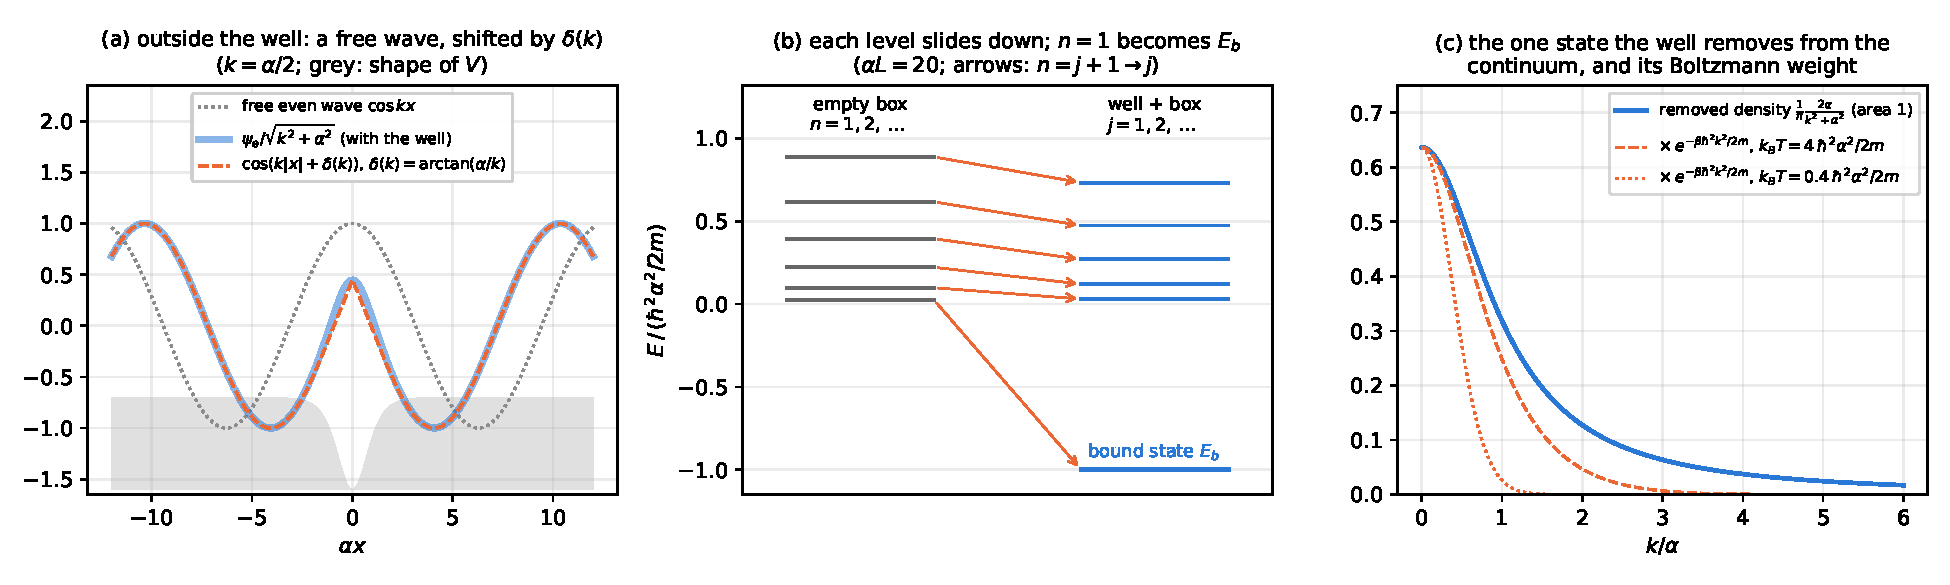
\includegraphics[width=\textwidth]{fig_explained_levels.pdf}
\caption{(a) The even solution \eqref{eq:psi} (blue) agrees outside the well with the free wave shifted by $\delta(k)$ (orange, dashed), \eqref{eq:farfield}. (b) Levels at $\alpha L=20$: each empty-box level $n=j+1$ slides down to $j$, and $n=1$ becomes the bound state. (c) The removed-state density of \eqref{eq:dos} (area 1), and its Boltzmann-weighted versions at two temperatures, as they enter $Z_q$ in \S\ref{sec:Zq}.}
\label{fig:levels}
\end{figure}

\subsection{A second route: associated Legendre functions}
\label{sec:legendre}
This is the route of most textbooks: a change of variable turns \eqref{eq:SE} into Legendre's equation, whose solutions are tabulated special functions. For $\lambda=2$ they reduce to the elementary functions of \S\ref{sec:solutions}.

\textbf{Step 1: the change of variable.} Let $t\equiv\tanh(\alpha x)\in(-1,1)$ and $\psi(x)=w(t)$.
\begin{align*}
\frac{\dd t}{\dd x}&=\frac{\alpha}{\cosh^2(\alpha x)}=\alpha(1-t^2) &&\why{F1a,b}\\
\psi'&=\frac{\dd t}{\dd x}\,w'(t)=\alpha(1-t^2)\,w' &&\why{chain rule}\\
\psi''&=\frac{\dd t}{\dd x}\,\frac{\dd}{\dd t}\Big[\alpha(1-t^2)w'\Big]=\alpha^2(1-t^2)\Big[(1-t^2)w''-2t\,w'\Big] &&\why{chain and product rules}
\end{align*}
Insert these into \eqref{eq:SE}, use $\frac{1}{\cosh^2(\alpha x)}=1-t^2$, and divide by $-\frac{\hbar^2\alpha^2}{2m}(1-t^2)$:
\begin{equation}
(1-t^2)\,w''-2t\,w'+\Big[\nu(\nu+1)-\frac{\mu^2}{1-t^2}\Big]w=0,\qquad \nu(\nu+1)=2\ \Rightarrow\ \nu=1,\qquad \mu^2\equiv-\frac{2mE}{\hbar^2\alpha^2}.
\label{eq:legendre}
\end{equation}
This is the associated Legendre equation, with \emph{degree} $\nu=1$ and \emph{order} $\mu$. (The other root, $\nu=-2$, gives the same equation.) The order depends on the energy:
\[
E=-\frac{\hbar^2\kappa^2}{2m}<0:\ \mu=\frac\kappa\alpha;\qquad E=0:\ \mu=0;\qquad E=\frac{\hbar^2k^2}{2m}>0:\ \mu=\frac{ik}{\alpha}\ \text{(imaginary)}.
\]
For general $\lambda$, $\nu(\nu+1)=\lambda(\lambda-1)$ gives $\nu=\lambda-1$. The walls $x=\pm\frac L2$ sit at $t=\pm\tL$, and the open line corresponds to $t\to\pm1$ \chk{C19}.
\src{The equation: [DLMF] 14.2.2. The $\mathrm{sech}^2$ well solved by an associated Legendre function of $\tanh x$: [LD, p.~3, Eqs.~(3.8)--(3.10)]. Their $u''+(E-\alpha\,\mathrm{sech}^2x)\,u=0$ is \eqref{eq:SE} in units $\hbar=2m=1$ with our $\alpha=1$, if their constant $\alpha$ (not ours) is $-2$; their degree $\frac12(\sqrt{1-4\alpha}-1)=1$ and order $i\sqrt E$ are our $\nu$ and $\mu$.}
\own{(standard) The derivation above.}

\textbf{Step 2: the Legendre function of degree 1 in closed form.} For $-1<t<1$ the (Ferrers) associated Legendre function is defined as
\[
\mathsf P_\nu^{\mu}(t)=\Big(\frac{1+t}{1-t}\Big)^{\mu/2}\frac{F\big(\nu+1,-\nu;1-\mu;\frac{1-t}{2}\big)}{\Gamma(1-\mu)} .
\]
For $\nu=1$ the second parameter is $-\nu=-1$, so the series stops after one term (F15):
\[
F\Big(2,-1;1-\mu;\frac{1-t}{2}\Big)=1-\frac{2}{1-\mu}\cdot\frac{1-t}{2}=\frac{t-\mu}{1-\mu}.
\]
Dividing by $\Gamma(1-\mu)$ and using $(1-\mu)\Gamma(1-\mu)=\Gamma(2-\mu)$ (F14):
\begin{equation}
\mathsf P_1^{\mu}(t)=\Big(\frac{1+t}{1-t}\Big)^{\mu/2}\frac{t-\mu}{\Gamma(2-\mu)},\qquad
\mathsf P_1^{-\mu}(t)=\Big(\frac{1-t}{1+t}\Big)^{\mu/2}\frac{t+\mu}{\Gamma(2+\mu)}.
\label{eq:P1}
\end{equation}
Because $1/\Gamma$ is finite everywhere (F14), \eqref{eq:P1} holds for every $\mu$, including $\mu=1$, where the factor $\frac{1}{1-\mu}$ alone would blow up. For $\mu=0$ it gives $\mathsf P_1(t)=t$. Substituting \eqref{eq:P1} directly into \eqref{eq:legendre} confirms that it is a solution, and it agrees with a library implementation for real and imaginary $\mu$ to 30 digits \chk{C19}.
\src{Definition: [DLMF] 14.3.1 with 14.3.3. $\mathsf P_1(t)=t$: [DLMF] 14.5.6.}
\own{The closed form \eqref{eq:P1} via the terminating series.}

\textbf{Step 3: a basis of solutions.} Equation \eqref{eq:legendre} is unchanged under $t\to-t$ (both $w''$ and $t\,w'$ keep their form), so $\mathsf P_1^{-\mu}(-t)$ is also a solution. Two solutions $f_1,f_2$ are independent when their Wronskian $f_1f_2'-f_1'f_2$ is nonzero: otherwise the $2\times2$ system $c_1f_1+c_2f_2=0$, $c_1f_1'+c_2f_2'=0$ has a nonzero solution $(c_1,c_2)$. Here
\[
\mathcal W\big\{\mathsf P_1^{-\mu}(t),\,\mathsf P_1^{-\mu}(-t)\big\}=\frac{2}{\Gamma(\mu-1)\,\Gamma(\mu+2)\,(1-t^2)} .
\]
By F14, $1/\Gamma(\mu-1)=0$ exactly when $\mu-1\in\{0,-1,-2,\dots\}$; with $\mathrm{Re}\,\mu\ge0$ that means $\mu=1$ or $\mu=0$ \chk{C19}.
\begin{itemize}
\item $\mu\neq0,1$ (every energy except $E=0$ and $E=-\Eu$): the general solution is $c_1\mathsf P_1^{-\mu}(t)+c_2\mathsf P_1^{-\mu}(-t)$.
\item $\mu=0$ ($E=0$) and $\mu=1$ ($E=-\Eu$): the two functions coincide up to sign, and a second solution ``of the second kind'' is needed. For $\mu=0$ it is $\mathsf Q_1(t)=\frac t2\ln\frac{1+t}{1-t}-1$; for $\mu=1$ it is $y_2$ of \eqref{eq:y12}.
\end{itemize}
That two independent solutions give all solutions is the standard theorem that the solutions of a linear second-order ODE form a two-dimensional space (no page-checked reference). In this document it also follows from \S\ref{sec:levels}.3.
\src{Wronskian: [DLMF] 14.2.3 with $\nu=1$. $\mathsf Q_1$: [DLMF] 14.5.8.}

\textbf{Step 4: back to $x$, the same functions as before.} By the definitions in F1,
$\frac{1-t}{1+t}=\frac{\cosh\alpha x-\sinh\alpha x}{\cosh\alpha x+\sinh\alpha x}=e^{-2\alpha x}$, so $\big(\frac{1-t}{1+t}\big)^{\mu/2}=e^{-\mu\alpha x}$. Then, from \eqref{eq:P1}:
\begin{itemize}
\item $E<0$, $\mu=\kappa/\alpha$. Using $e^{\mp\kappa x}=\cosh\kappa x\mp\sinh\kappa x$ in \eqref{eq:chi},
\begin{align*}
\alpha\,\Gamma\big(2+\tfrac\kappa\alpha\big)\,\mathsf P_1^{-\kappa/\alpha}(\tanh\alpha x)&=(\kappa+\alpha\tanh\alpha x)\,e^{-\kappa x}=\chi_e+\chi_o,\\
\alpha\,\Gamma\big(2+\tfrac\kappa\alpha\big)\,\mathsf P_1^{-\kappa/\alpha}(-\tanh\alpha x)&=(\kappa-\alpha\tanh\alpha x)\,e^{\kappa x}=\chi_e-\chi_o .
\end{align*}
\item $E>0$, $\mu=ik/\alpha$. Using $e^{-ikx}=\cos kx-i\sin kx$ (F13),
\[
\alpha\,\Gamma\big(2+\tfrac{ik}\alpha\big)\,\mathsf P_1^{-ik/\alpha}(\tanh\alpha x)=(\alpha\tanh\alpha x+ik)\,e^{-ikx}=\psi_o+i\,\psi_e .
\]
The equation has real coefficients, so the real and imaginary parts, $\psi_o$ and $\psi_e$ of \eqref{eq:psi}, are solutions themselves (F13).
\item $E=0$, $\mu=0$: $\mathsf P_1=\tanh\alpha x$ and, since $\ln\frac{1+t}{1-t}=2\alpha x$, $\mathsf Q_1=\alpha x\tanh\alpha x-1$. These are the two solutions of \S\ref{sec:solutions}(b).
\item $E=-\Eu$, $\mu=1$: $\mathsf P_1^{-1}(t)=\frac12\sqrt{1-t^2}=\frac{1}{2\cosh\alpha x}=\frac12y_1$, and the second solution is $y_2$ of \eqref{eq:y12}.
\end{itemize}
So both routes give identical functions \chk{C19}, and the box analysis of \S\ref{sec:walls} applies unchanged.
\own{Step 4.}

\textbf{Step 5: where the boundary conditions enter.} A Legendre function by itself carries no boundary condition: it is just a solution of \eqref{eq:legendre}. The boundary condition picks the combination and the allowed energies.
\begin{itemize}
\item \emph{Box (our problem):} $w=0$ at $t=\pm\tL$. Since the functions are those of \S\ref{sec:solutions}, this gives exactly the conditions \eqref{eq:quant} and \eqref{eq:bound}.
\item \emph{Open line, $\psi\to0$ as $x\to\pm\infty$, i.e.\ as $t\to\pm1$, for $E<0$ ($\mu>0$):} as $t\to1$, $\mathsf P_1^{-\mu}(t)\propto(1-t)^{\mu/2}\to0$. As $t\to-1$, the factor $\big(\frac{1-t}{1+t}\big)^{\mu/2}$ diverges, and the other factor tends to $t+\mu\to\mu-1$. So $\mathsf P_1^{-\mu}(t)\to\infty$ unless $\mu=1$; for $\mu=1$ it is $\frac12\sqrt{1-t^2}\to0$. The partner $\mathsf P_1^{-\mu}(-t)$ is the mirror image. In a combination $c_1\mathsf P_1^{-\mu}(t)+c_2\mathsf P_1^{-\mu}(-t)$ that vanishes at both ends, the behaviour near $t=1$ forces $c_2=0$ and near $t=-1$ forces $c_1=0$, unless $\mu=1$ \chk{C19}. Hence the open line has exactly one bound state: $\mu=1$, i.e.\ $E=-\Eu$, $\psi\propto1/\cosh(\alpha x)$, as in [CKS, p.~78].
\end{itemize}
\own{Step 5.}

\subsection{Which route is better? A recommendation}
\label{sec:routes}
\begin{center}
\small
\begin{tabular}{p{0.2\textwidth}p{0.36\textwidth}p{0.36\textwidth}}
\toprule
 & Factorization (SUSY), \S\ref{sec:levels}.1--\ref{sec:walls} & Associated Legendre, \S\ref{sec:legendre}\\
\midrule
Mathematics needed & derivatives, product rule, linear maps (F3--F5) & also complex orders, $\Gamma$, hypergeometric series, Ferrers functions (F13--F15)\\
All solutions found? & yes, by a linear-algebra argument (\S\ref{sec:levels}.3) & yes, via a tabulated Wronskian plus the two-dimensional-solution-space theorem\\
Exceptional energies & one: $E=-\Eu$ & two: $E=0$ and $E=-\Eu$ (second-kind functions needed)\\
Phase shift, ``reflectionless'', one state removed & immediate: $\Ad$ maps the free wave to the shifted wave \eqref{eq:farfield} & only after reducing $\mathsf P_1^{-\mu}$ to elementary form\\
Which $\lambda$ & integer $\lambda$ (the chain of partners ends at the free particle); $\lambda=2$ needs one step & any $\lambda$, integer or not, from one formula ($\nu=\lambda-1$)\\
\bottomrule
\end{tabular}
\end{center}

\textbf{General $\lambda$, for reference.} For general $\lambda$ the Legendre route gives open-line bound states at $\mu=\nu-n$, i.e.
$E_n=-\frac{\hbar^2\alpha^2}{2m}(\lambda-1-n)^2$ for $n=0,1,\dots$ with $n<\lambda-1$. This is stated here without proof. It is checked by finite differences for $\lambda=2,\ 2.5,\ 3$ \chk{C19}, and for $\lambda=3$ it matches ``$V_1=-6\,\mathrm{sech}^2x$ \dots\ two bound states at $E_1=-4$ and $E_2=-1$'' [CKS, p.~78]. No page-checked source was found for general $\lambda$.

\begin{result}
\textbf{Recommendation} (Claude's own judgement).
\begin{enumerate}[label=\arabic*.]
\item \emph{For this project ($\lambda=2$, hard walls), use the factorization (SUSY) route as the main derivation.}
\begin{itemize}
\item It needs only Calculus~1 and linear algebra.
\item It proves within itself that all solutions have been found.
\item Its first output, $\Ad$ applied to a free wave, is already the phase-shifted wave \eqref{eq:farfield}. That gives $\delta(k)$ and the level density \eqref{eq:dos}, which are exactly what $Z_q$ needs in \S\ref{sec:Zq}.
\end{itemize}
\item \emph{Keep the Legendre route as an independent cross-check.} It reproduces every function (C19), so nothing is lost by not using it as the main line.
\item \emph{Switch to the Legendre route if the project moves to non-integer $\lambda$}, i.e.\ to a continuously tunable well depth at fixed width.
\begin{itemize}
\item Then the chain of partners no longer ends at the free particle (compare [CKS, pp.~41--42], integer case), so there are no elementary solutions, and the reflectionless property used in \S\ref{sec:phase} is lost.
\item The box conditions must then be evaluated with $\mathsf P_\nu^{\pm\mu}(\pm t)$ numerically (for example \texttt{mpmath.legenp}).
\item For integer $\lambda>2$ both routes work: SUSY needs $\lambda-1$ factorization steps, while Legendre gives everything in one terminating formula.
\end{itemize}
\end{enumerate}
\end{result}
\own{The comparison and the recommendation.}

% =====================================================================
\section{The quantum partition function}
\label{sec:Zq}
By P3 and \S\ref{sec:levels},
\begin{equation}
Z_q=e^{-\beta E_b}+\sum_{j\ge1}e^{-\beta E_j}.
\label{eq:Zqsum}
\end{equation}
From here on, $\alpha\tL$ and $\kappa_b$ are replaced by $\alpha$ (A3). The exact version keeps them; it is Eq.~\eqref{eq:Zqexact} below.

\subsection{From the sum to an integral}
Let $y(k)\equiv\big[kL-2\arctan\frac k\alpha\big]/\pi$, so that $y(k_j)=j$ by \eqref{eq:quant}. Then $y$ is odd (F2a), $y(0)=0$, and $y'(k)=\big[L-\frac{2\alpha}{k^2+\alpha^2}\big]/\pi>0$. So $y$ has a smooth, odd inverse $k(y)$, with $k'(y)=1/y'(k(y))$ (inverse-function rule). Define
\begin{equation}
F(y)\equiv\exp\Big(-\frac{\beta\hbar^2k(y)^2}{2m}\Big).
\label{eq:F}
\end{equation}
Then $F(j)=e^{-\beta E_j}$, $F$ is smooth and even (because $k(-y)^2=k(y)^2$), $F(0)=1$, and $F$ decays like a Gaussian. By F10,
\begin{equation}
\sum_{j\ge1}e^{-\beta E_j}=\int_0^\infty F(y)\,\dd y-\frac12+R .
\label{eq:sum2int}
\end{equation}
\own{Applying F10 to this sum.}

\textbf{How small is $R$? (A4)}
\begin{itemize}
\item \emph{Empty box.} Here $F(y)=e^{-\beta E_1y^2}$ with $\beta E_1=\frac{\pi\lth^2}{4L^2}$ (using $\frac{\beta\hbar^2}{m}=\frac{\lth^2}{2\pi}$). Then \eqref{eq:Rgauss} gives
\begin{equation}
R=\frac{2L}{\lth}\sum_{\ell\ge1}e^{-4\pi\ell^2(L/\lth)^2}:\qquad 7.0\times10^{-6},\ \ 5.9\times10^{-22},\ \ 4.6\times10^{-49}\ \ \text{at}\ \ L/\lth=1,\,2,\,3\ \chk{C9a}.
\label{eq:Rbox}
\end{equation}
\item \emph{Well + box}, computed from the exact levels at 80 digits \chk{C9b}: $R$ equals \eqref{eq:Rbox} plus a part that is at most $4(\alpha L)^2e^{-2\alpha L}$ times the bound-state weight $e^{a/2}$, in all nine cases computed ($\alpha L=20,30,60$; $L/\lth=1,2,3$).
\item In the anomaly windows of \S\ref{sec:compare}, $L/\lth\ge10$, where the empty-box part is below $10^{-500}$. That dropping $R$ is harmless there is also checked directly: $\Cq$ from the closed form agrees with the exact level sum to $2\times10^{-13}\kB$ \chk{C13}.
\end{itemize}
\own{The size of $R$ for the well. This is a numerical observation: estimating it analytically needs complex analysis, and no reference was found.}

\subsection{Change of variables, and the two integrals}
Substitute $y=y(k)$, $\dd y=y'(k)\,\dd k$ ($k$ runs from $0$ to $\infty$ as $y$ does), and use F6 and F11 with $s=\frac{\beta\hbar^2}{2m}$ and $c=\alpha$:
\begin{align}
\int_0^\infty F(y)\,\dd y&=\frac{L}{\pi}\int_0^\infty e^{-\beta\hbar^2k^2/2m}\,\dd k-\frac{2\alpha}{\pi}\int_0^\infty\frac{e^{-\beta\hbar^2k^2/2m}}{k^2+\alpha^2}\,\dd k \nonumber\\
&=\frac{L}{\pi}\cdot\frac12\sqrt{\frac{2\pi m}{\beta\hbar^2}}-\frac{2\alpha}{\pi}\cdot\frac{\pi}{2\alpha}\,e^{\beta\hbar^2\alpha^2/2m}\erfc\sqrt{\frac{\beta\hbar^2\alpha^2}{2m}}
=\frac{L}{\lth}-e^{a/2}\erfc\sqrt{a/2}.
\label{eq:twoint}
\end{align}
The last step uses $\frac{L}{2\pi}\sqrt{\frac{2\pi m}{\beta\hbar^2}}=L\sqrt{\frac{m}{2\pi\hbar^2\beta}}=\frac{L}{\lth}$ and $\frac{\beta\hbar^2\alpha^2}{2m}=\frac a2$.
\own{Eq.~\eqref{eq:twoint}.}

\subsection{The closed form}
Insert \eqref{eq:sum2int} and \eqref{eq:twoint} into \eqref{eq:Zqsum}, with $e^{-\beta E_b}=e^{a/2}$, and use $1-\erfc=\erf$:
\begin{result}
\begin{equation}
Z_q=\frac{L}{\lth}-\frac12+e^{a/2}\erf\sqrt{a/2},\qquad a=\frac{\beta\hbar^2\alpha^2}{m},\quad \frac{L}{\lth}=\frac{\alpha L}{\sqrt{2\pi a}}.
\label{eq:Zq}
\end{equation}
\end{result}
\emph{Exact version} (A3 not used): keep $\alpha\tL$ in \eqref{eq:twoint} and $\kappa_b$ in the bound state,
\begin{equation}
Z_q=\frac{L}{\lth}-\frac12+e^{\beta\hbar^2\kappa_b^2/2m}-e^{\beta\hbar^2\alpha^2\tanh^2(\alpha L/2)/2m}\,\erfc\sqrt{\frac{\beta\hbar^2\alpha^2\tanh^2(\alpha L/2)}{2m}}+R .
\label{eq:Zqexact}
\end{equation}
Without $R$, \eqref{eq:Zqexact} and \eqref{eq:Zq} both equal the direct level sum to $2\times10^{-16}$ (relative) at $\alpha L=100$ \chk{C11}. Replacing $\kappa_b$ by $\alpha$ changes the bound-state exponent by $\frac{\beta\hbar^2(\alpha^2-\kappa_b^2)}{2m}\approx4a\,e^{-\alpha L}$, by \eqref{eq:Eb}.
\own{Eqs.~\eqref{eq:Zqsum}--\eqref{eq:Zqexact}. No reference found for this closed form.}

\begin{intuition}
\[
Z_q=\underbrace{\frac{L}{\lth}}_{\text{free particle}}\ \underbrace{-\ \frac12}_{\text{hard walls}}\ +\ \underbrace{e^{a/2}}_{\text{bound state}}\ \underbrace{-\ e^{a/2}\erfc\sqrt{a/2}}_{\text{the continuum state the well removed}}.
\]
\begin{itemize}
\item $L/\lth$: the number of thermal wavelengths in the box (P5).
\item $-\frac12$: in \eqref{eq:sum2int}, the integral includes the point $j=0$ with weight $F(0)/2=\frac12$ (Step~1 of F10), but $j=0$ ($k=0$) is not a level (\S\ref{sec:walls}~(ii)); the $-\frac12$ removes it. Equivalently, $\frac{L}{\lth}-\frac12=\frac{L-\lth/2}{\lth}$: each wall makes a layer $\lth/4$ unavailable.
\item $e^{a/2}=e^{-\beta E_b}$: the bound state.
\item The last term equals $\int_0^\infty\frac1\pi\frac{2\alpha}{k^2+\alpha^2}e^{-\beta\hbar^2k^2/2m}\dd k$ (F11): the Boltzmann weight of the state removed in \eqref{eq:dos}, which is spread over $k\lesssim\alpha$ (Fig.~\ref{fig:levels}c). At high $T$ ($a\to0$) it counts fully, tending to $1$, and cancels the bound state: the well no longer matters. At low $T$ ($a\to\infty$) only $\approx\sqrt{2/\pi a}$ of it is thermally reachable (F7d).
\end{itemize}
\end{intuition}
\own{This reading.}

% =====================================================================
\section{The quantum heat capacity}
\label{sec:Cq}
Use P4(d) with $a=\frac{\hbar^2\alpha^2}{m}\beta$. Write $Z_q=B(a)-\frac12+G(a)$, where
$B\equiv\frac{L}{\lth}=\frac{\alpha L}{\sqrt{2\pi a}}$ and $G\equiv e^{a/2}\erf\sqrt{a/2}$. The derivatives (${}'=\dd/\dd a$) are:
\begin{align}
B&\propto a^{-1/2}: && B'=-\frac{B}{2a},\qquad B''=\frac{3B}{4a^2}, \label{eq:Bder}\\
G'&=\frac12e^{a/2}\erf\sqrt{a/2}+e^{a/2}\,\frac{e^{-a/2}}{\sqrt{2\pi a}}=\frac G2+\frac{1}{\sqrt{2\pi a}} && \why{product rule, F7b} \label{eq:G1}\\
G''&=\frac{G'}2-\frac{1}{2\sqrt{2\pi}}\,a^{-3/2}. && \label{eq:G2}
\end{align}
\chk{C12}
\begin{result}
\begin{equation}
\frac{\Cq}{\kB}=a^2\left[\frac{B''+G''}{B-\frac12+G}-\left(\frac{B'+G'}{B-\frac12+G}\right)^2\right],\qquad a=\frac{\beta\hbar^2\alpha^2}{m}.
\label{eq:Cq}
\end{equation}
\end{result}
Only $\alpha L$ and $a$ appear, as \eqref{eq:dimless} requires. For numerics, multiply $Z_q$, $Z_q'$ and $Z_q''$ by $e^{-a/2}$; the ratios do not change and nothing overflows. Against $\kB\beta^2\mathrm{Var}(E)$ over the exact levels, \eqref{eq:Cq} agrees to $2\times10^{-13}\kB$ for $\alpha L=60,100,1000$ and $\kB T\in[0.02,5]$ \chk{C13}.

\textbf{Low $T$} ($a\to\infty$). Let $Z_c\equiv\sum_{j\ge1}e^{-\beta E_j}=\frac{L}{\lth}-\frac12-e^{a/2}\erfc\sqrt{a/2}$ be the continuum part, so $Z_q=e^{a/2}(1+u)$ with $u=Z_ce^{-a/2}\ll1$. Then $\ln Z_q=\frac a2+\ln(1+u)\approx\frac a2+u$, and since $Z_c\propto a^{-1/2}$ to leading order,
\begin{equation}
\Cq\approx\kB\,a^2u''=\kB\Big(\frac a2\Big)^2Z_c\,e^{-a/2}\Big[1+\frac2a+\dots\Big]\ \longrightarrow\ 0\quad\text{(exponentially)}.
\label{eq:Cqlow}
\end{equation}
This is the two-level form P4(f), with gap $\Delta=\Eu$ (so $\beta\Delta=a/2$) and the whole continuum acting as one excited level of ``degeneracy'' $Z_c$ \chk{C13: ratio $1.0151$ at $a=160$, against $1+2/a=1.0125$}.

\textbf{High $T$} ($a\to0$): see \S\ref{sec:highT}.
\own{Eqs.~\eqref{eq:Bder}--\eqref{eq:Cqlow}.}

% =====================================================================
\section{The classical partition function and heat capacity}
\label{sec:classical}

\subsection{Partition function}
By P5, over the box, with $-\beta V(x)=\frac{a}{\cosh^2(\alpha x)}$ from \eqref{eq:V}:
\begin{equation}
Z_{\rm cl}=\frac{1}{\lth}\int_{-L/2}^{L/2}e^{a/\cosh^2(\alpha x)}\,\dd x .
\label{eq:Zcl0}
\end{equation}
Split off the flat part, writing $e^{a/\cosh^2}=1+\big(e^{a/\cosh^2}-1\big)$, and extend the second integral to all $x$:
\begin{equation}
Z_{\rm cl}=\frac{L+I}{\lth}=\frac{\alpha L+\alpha I}{\sqrt{2\pi a}},\qquad I\equiv\int_{-\infty}^{\infty}\Big(e^{a/\cosh^2(\alpha x)}-1\Big)\dd x .
\label{eq:Zcl}
\end{equation}
\emph{Error of the extension (A3).} For $|x|\ge\frac L2$, $v\equiv\frac{a}{\cosh^2(\alpha x)}\le v_0\equiv4ae^{-\alpha L}$ (F1e), and $e^v-1\le v\,e^{v_0}$. So the two added tails total at most $2e^{v_0}\frac a\alpha\big(1-\tL\big)<\frac{4a}{\alpha}e^{-\alpha L}e^{v_0}$, which is $3\times10^{-42}/\alpha$ at $\alpha L=100$, $a=20$ \chk{C14}.

\subsection{The well integral}
Substitute $t=\tanh(\alpha x)$. Then $\dd t=\frac{\alpha}{\cosh^2(\alpha x)}\dd x=\alpha(1-t^2)\,\dd x$ (F1a,b), $\frac{1}{\cosh^2(\alpha x)}=1-t^2$, and $x\in(-\infty,\infty)$ maps to $t\in(-1,1)$:
\begin{equation}
\alpha I=\int_{-1}^{1}\frac{e^{a(1-t^2)}-1}{1-t^2}\,\dd t .
\label{eq:It}
\end{equation}
The integrand is continuous on $[-1,1]$, since $(e^{av}-1)/v\to a$ as $v\to0$.

\emph{Series.} $\frac{e^{av}-1}{v}=\sum_{\ell\ge1}\frac{a^\ell v^{\ell-1}}{\ell!}$ converges uniformly for $v=1-t^2\in[0,1]$ (F9). Integrating term by term with F12 ($n=\ell-1$):
\begin{equation}
\alpha I=\sum_{\ell\ge1}\frac{a^\ell}{\ell!}\int_{-1}^{1}(1-t^2)^{\ell-1}\dd t=\sum_{\ell\ge1}\frac{a^\ell}{\ell!}\cdot\frac{2^\ell(\ell-1)!}{(2\ell-1)!!}=\sum_{\ell\ge1}\frac{(2a)^\ell}{\ell\,(2\ell-1)!!}=2a+\frac{2a^2}{3}+\frac{8a^3}{45}+\dots
\label{eq:Iseries}
\end{equation}
It converges for every $a$: the ratio of successive terms is $\frac{2a\,\ell}{(\ell+1)(2\ell+1)}\to0$. It agrees with \eqref{eq:It} to $2\times10^{-15}$ \chk{C14}.

\subsection{Derivatives in \texorpdfstring{$a$}{a}}
By F8,
\begin{align}
\alpha J_1\equiv\frac{\dd(\alpha I)}{\dd a}&=\int_{-1}^{1}e^{a(1-t^2)}\dd t=2e^a\int_0^1e^{-at^2}\dd t=\frac{2e^a}{\sqrt a}\int_0^{\sqrt a}e^{-u^2}\dd u=\sqrt\pi\,\frac{e^a\erf\sqrt a}{\sqrt a}, \label{eq:J1}\\
\alpha J_2\equiv\frac{\dd(\alpha J_1)}{\dd a}&=\int_{-1}^{1}(1-t^2)\,e^{a(1-t^2)}\dd t=\alpha J_1\Big(1-\frac{1}{2a}\Big)+\frac1a . \label{eq:J2}
\end{align}
In \eqref{eq:J1} the integrand is even, $u=\sqrt a\,t$, and F7 is used. The last form of \eqref{eq:J2} comes from differentiating \eqref{eq:J1} with the product rule and F7b: $\frac{\dd}{\dd a}\big[\sqrt\pi\,e^aa^{-1/2}\erf\sqrt a\big]=\alpha J_1\big(1-\frac1{2a}\big)+\sqrt\pi\,e^aa^{-1/2}\frac{e^{-a}}{\sqrt{\pi a}}$ \chk{C12, C14}. Undoing $t=\tanh(\alpha x)$,
\begin{equation}
J_1=\int\frac{e^{a/\cosh^2(\alpha x)}}{\cosh^2(\alpha x)}\,\dd x,\qquad J_2=\int\frac{e^{a/\cosh^2(\alpha x)}}{\cosh^4(\alpha x)}\,\dd x .
\label{eq:Jx}
\end{equation}

\subsection{Heat capacity}
From \eqref{eq:Zcl}, $\ln Z_{\rm cl}=\ln(\alpha L+\alpha I)-\frac12\ln(2\pi a)$. In P4(d):
$a^2\frac{\dd^2}{\dd a^2}\big[-\frac12\ln(2\pi a)\big]=a^2\cdot\frac{1}{2a^2}=\frac12$, and
$\frac{\dd}{\dd a}\ln(\alpha L+\alpha I)=\frac{\alpha J_1}{\alpha L+\alpha I}$, $\frac{\dd^2}{\dd a^2}\ln(\alpha L+\alpha I)=\frac{\alpha J_2}{\alpha L+\alpha I}-\Big(\frac{\alpha J_1}{\alpha L+\alpha I}\Big)^2$. Hence
\begin{result}
\begin{equation}
\frac{\Ccl}{\kB}=\frac12+a^2\left[\frac{\alpha J_2}{\alpha L+\alpha I}-\left(\frac{\alpha J_1}{\alpha L+\alpha I}\right)^2\right],
\qquad \alpha I\text{ from \eqref{eq:Iseries}},\ \ \alpha J_1,\ \alpha J_2\text{ from \eqref{eq:J1}--\eqref{eq:J2}}.
\label{eq:Ccl}
\end{equation}
\end{result}
\begin{intuition}
This is \eqref{eq:Cclsplit}. The $\frac12$ is the kinetic energy (equipartition). By \eqref{eq:Jx}, $\langle1/\cosh^2\rangle=J_1/(L+I)$ and $\langle1/\cosh^4\rangle=J_2/(L+I)$ under $P(x)\propto e^{-\beta V(x)}$, so the bracket is $\mathrm{Var}\big(1/\cosh^2(\alpha x)\big)$, and $a^2\,\mathrm{Var}(1/\cosh^2)=\beta^2\mathrm{Var}(V)$. Formula \eqref{eq:Ccl} agrees with a direct numerical integration of \eqref{eq:Cclsplit} to $10^{-9}\kB$ \chk{C14}.
\end{intuition}

\textbf{Limits.}
\emph{Low $T$} ($a\to\infty$): near $x=0$, $\frac{1}{\cosh^2(\alpha x)}=1-\alpha^2x^2+O(x^4)$, so $V\approx-\frac{\hbar^2\alpha^2}{m}+\frac{\hbar^2\alpha^4}{m}x^2$, a harmonic oscillator with $\frac12m\omega_0^2=\frac{\hbar^2\alpha^4}{m}$. By equipartition (P5), $\Ccl\to\kB$; the next order is $\Ccl\approx\kB(1+1/a)$ \chk{C14: $1.001004$ at $a=1000$}. In the same limit, $e^{a(1-t^2)}\approx e^ae^{-at^2}$ gives $\alpha I\approx e^a\sqrt{\pi/a}$ (F6).
\emph{High $T$} ($a\to0$): $a^2\,\mathrm{Var}\to0$, so $\Ccl\to\kB/2$.
\own{Eqs.~\eqref{eq:Zcl0}--\eqref{eq:Ccl} and the limits, by standard techniques. No reference found for \eqref{eq:Iseries}--\eqref{eq:Ccl} for this potential.}

% =====================================================================
\section{Comparing \texorpdfstring{$\Cq$}{Cq} and \texorpdfstring{$\Ccl$}{Ccl}}
\label{sec:compare}

\subsection{An exact relation between \texorpdfstring{$Z_q$}{Zq} and \texorpdfstring{$Z_{\rm cl}$}{Zcl}}
By F7c with $z^2=a/2$ (so $2^nz^{2n}=a^n$), $G=e^{a/2}\erf\sqrt{a/2}=\sqrt{\frac{2a}{\pi}}\sum_{n\ge0}\frac{a^n}{(2n+1)!!}$. By \eqref{eq:Iseries} with $\ell=n+1$, $\frac{I}{\lth}=\frac{\alpha I}{\sqrt{2\pi a}}=\sqrt{\frac{2a}{\pi}}\sum_{n\ge0}\frac{2^n}{n+1}\frac{a^n}{(2n+1)!!}$. Subtracting, $Z_q-Z_{\rm cl}=-\frac12+G-\frac{I}{\lth}$, so
\begin{equation}
Z_q=Z_{\rm cl}-\frac12-D(a),\qquad D(a)\equiv\sqrt{\frac{2a}{\pi}}\sum_{n\ge2}\Big(\frac{2^n}{n+1}-1\Big)\frac{a^n}{(2n+1)!!}=\sqrt{\frac{2a}{\pi}}\Big(\frac{a^2}{45}+\frac{a^3}{105}+\dots\Big)>0 .
\label{eq:exact}
\end{equation}
The terms $n=0,1$ cancel exactly, and every coefficient with $n\ge2$ is positive because $2^n>n+1$ \chk{C15}. So at every $T$ the quantum particle has \emph{less} weight in the well than the classical one ($D>0$, the zero-point cost), and the walls remove another $\frac12$.
\own{Eq.~\eqref{eq:exact}. No reference found.}

\subsection{High temperature}
\label{sec:highT}
For $a\to0$, $Z_{\rm cl}\approx L/\lth\gg\frac12+D$, so $\ln Z_q-\ln Z_{\rm cl}=\ln\big(1-\frac{1/2+D}{Z_{\rm cl}}\big)\approx-\frac{\lth}{2L}-\frac{\lth}{L}D$. Apply the sign rule P4(e) to each term:
\begin{itemize}
\item \emph{Walls:} $-\frac{\lth}{2L}\propto\beta^{1/2}$, so $p=\frac12$:
\begin{equation}
\Cq-\Ccl\ \xrightarrow{\;T\to\infty\;}\ \kB\,\frac{\lth}{8L}>0 .
\label{eq:wall}
\end{equation}
\item \emph{Well:} $-\frac{\lth}{L}D\approx-\frac{\sqrt{2\pi a}}{\alpha L}\sqrt{\frac{2a}\pi}\frac{a^2}{45}=-\frac{2a^3}{45\,\alpha L}\propto\beta^3$, so $p=3$, contributing $-\frac{4}{15}\frac{a^3}{\alpha L}\,\kB<0$.
\end{itemize}
At high $T$ the walls give the only excess, and the smooth well gives a deficit. At $\kB T=2000\,\Eu$ ($a=0.001$) and $\alpha L=100$: $\Cq-\Ccl=9.9089\times10^{-5}\kB$, against $\lth/8L=9.9083\times10^{-5}$ \chk{C15}.
\own{This subsection.}

\subsection{The empty box: the wall effect alone}
\label{sec:box}
Without the well, \eqref{eq:boxlevels} and \eqref{eq:Rbox} give $Z_q=y-\frac12+R$ with $y\equiv L/\lth\propto\beta^{-1/2}$. Classically $Z_{\rm cl}=y$ exactly, so $\Ccl=\kB/2$ at every $T$. Drop $R$ and use $\beta y'=-\frac y2$ and $\beta^2y''=\frac34y$ (${}'=\dd/\dd\beta$) in \eqref{eq:Cv}:
\begin{align*}
\frac{\Cq}{\kB}&=\beta^2\left[\frac{y''}{y-\frac12}-\left(\frac{y'}{y-\frac12}\right)^2\right]=\frac{\frac34y\big(y-\frac12\big)-\frac14y^2}{\big(y-\frac12\big)^2}=\frac{y\big(2y-\frac32\big)}{4\big(y-\frac12\big)^2},
\end{align*}
and subtracting $\frac12$:
\begin{result}
\begin{equation}
\frac{\Cq-\Ccl}{\kB}=\frac{y-1}{8\big(y-\frac12\big)^2}=\frac{r(1-r)}{2(2-r)^2},\qquad r\equiv\frac{\lth}{L}=\frac1y .
\label{eq:boxexcess}
\end{equation}
\end{result}
\begin{itemize}
\item It is positive iff $r<1$, i.e.\ $L>\lth$, i.e.\ $\kB T>\frac4\pi E_1$ (using $r^2=\frac{4}{\pi}\frac{E_1}{\kB T}$).
\item $\frac{\dd}{\dd r}\frac{r(1-r)}{(2-r)^2}=\frac{2-3r}{(2-r)^3}$ vanishes at $r=\frac23$, so the maximum is $\frac{(2/3)(1/3)}{2(4/3)^2}=\frac{1}{16}$, at $\kB T=\frac9\pi E_1\approx2.865E_1$.
\item As $T\to\infty$ it tends to $\frac r8=\frac{\lth}{8L}$, the wall term \eqref{eq:wall}.
\end{itemize}
Against the exact level sum: the exact maximum is $0.562500\kB$ at $2.864E_1$, and the excess starts at $1.265E_1$ (the formula gives $\frac4\pi=1.273$). Formula \eqref{eq:boxexcess} is good to $10^{-9}$ for $r<\frac23$ \chk{C16}. Inside the anomaly windows below, $r\le0.1$, so this term is at most $0.013\kB$.
\src{That $\Cq>\Ccl$ for a particle in a 1D box: [LGK, p.~95, Fig.~4.3 (right); p.~96].}
\own{Eq.~\eqref{eq:boxexcess} and its analysis.}
\begin{intuition}
$Z_q=(L-\lth/2)/\lth$: the walls exclude a layer $\lth/4$ each. Heating shrinks the layer ($\lth\propto T^{-1/2}$) and gives the particle room, and that costs extra energy, hence extra heat capacity.
\end{intuition}

\begin{figure}[h]
\centering
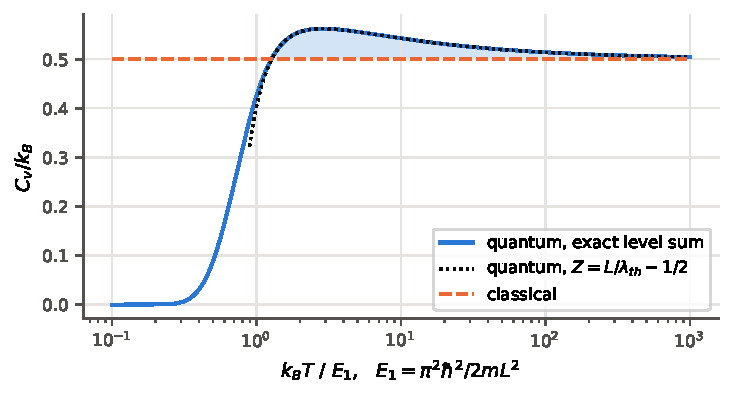
\includegraphics[width=0.62\textwidth]{fig_box_only.pdf}
\caption{Empty box: exact level sum (blue), Eq.~\eqref{eq:boxexcess} (dotted) and the classical $\kB/2$ (orange, dashed), against $\kB T/E_1$.}
\label{fig:box}
\end{figure}

\subsection{The numbers}
Table~\ref{tab:anomaly} evaluates the closed forms \eqref{eq:Cq} and \eqref{eq:Ccl}, with no further approximation, on 20\,000 temperatures in $\kB T\in[0.02,1]$ \chk{C17}. There is no closed-form proof here that $\Cq>\Ccl$ somewhere: the windows are found by evaluating the two formulas.
\begin{table}[h]
\centering
\caption{Quantum against classical heat capacity. $\kB T$ in units of $\Eu$; ``window'' is where $\Cq>\Ccl$.}
\label{tab:anomaly}
\resizebox{\textwidth}{!}{%
\begin{tabular}{cccccccc}
\toprule
$\alpha L$ & $\max(\Cq-\Ccl)/\kB$ & at $\kB T$ & $\Cq/\kB$, $\Ccl/\kB$ there & window & $\Cq$ peak (at) & $\Ccl$ peak (at) & $\min(\Cq-\Ccl)/\kB$ (at)\\
\midrule
30 & none for $\kB T<1$ & -- & -- & -- & 2.00 (0.393) & 3.74 (0.412) & $-1.75$ (0.421)\\
70 & $-0.039$ (none) & 0.216 & 1.906, 1.946 & -- & 3.04 (0.310) & 5.40 (0.363) & $-2.65$ (0.386)\\
80 & $+0.095$ & 0.214 & 2.093, 1.997 & $[0.195,0.231]$ & 3.23 (0.300) & 5.69 (0.356) & $-2.84$ (0.379)\\
100 & $+0.343$ & 0.210 & 2.427, 2.084 & $[0.176,0.239]$ & 3.56 (0.285) & 6.21 (0.344) & $-3.18$ (0.367)\\
400 & $+2.591$ & 0.184 & 5.091, 2.499 & $[0.129,0.223]$ & 6.05 (0.216) & 10.03 (0.283) & $-6.20$ (0.299)\\
1000 & $+4.802$ & 0.167 & 7.397, 2.595 & $[0.112,0.203]$ & 8.13 (0.185) & 13.13 (0.252) & $-9.10$ (0.263)\\
\bottomrule
\end{tabular}}
\end{table}

\begin{figure}[h]
\centering
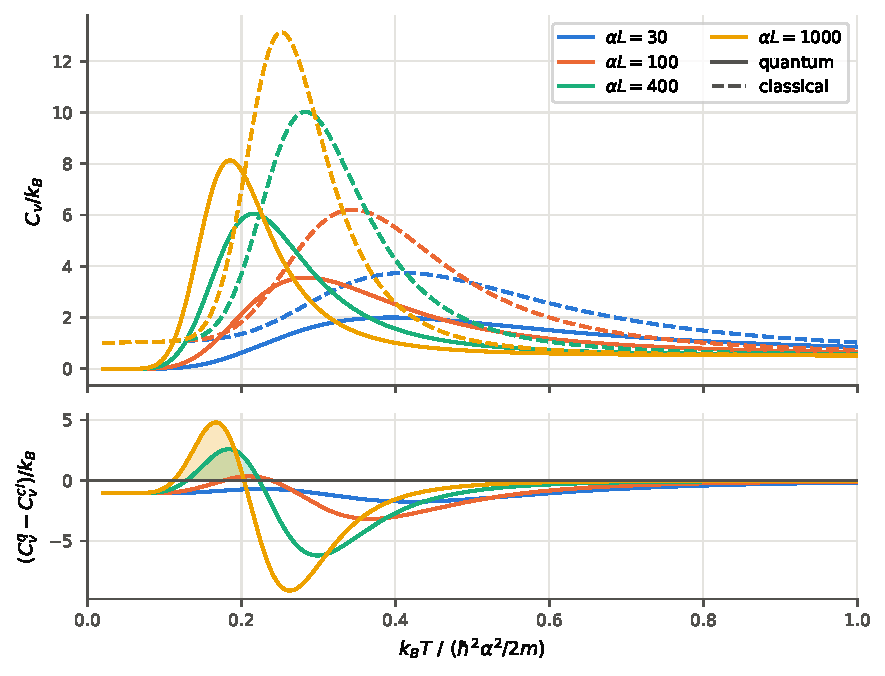
\includegraphics[width=0.78\textwidth]{fig_cv_cases.pdf}
\caption{$\Cq$ (solid) and $\Ccl$ (dashed), and their difference, for four box lengths. Shaded: $\Cq>\Ccl$.}
\label{fig:cases}
\end{figure}

\subsection{Why there is a window (heuristic, not a proof)}
\label{sec:heuristic}
Each $C_v$ curve is dominated by one event: the particle leaving the well for the box (desorption). Treat it as a two-level system, P4(f), with ``bound'' and ``free'' weights:
\begin{itemize}
\item quantum: bound $e^{a/2}$ ($=e^{-\beta E_b}$), free $L/\lth$;
\item classical: bound $I/\lth\approx\frac{e^a}{\sqrt2\,a}$ (from $\alpha I\approx e^a\sqrt{\pi/a}$ and $\alpha\lth=\sqrt{2\pi a}$), free $L/\lth$. Here $e^a=e^{-\beta V_{\min}}$ and $\frac{1}{\sqrt2\,a}=\frac{\kB T}{\hbar\omega_0}$ is the oscillator partition function of the bottom [Tong-SP, p.~47, Eq.~(2.20)], with $\hbar\omega_0=\sqrt2\,\hbar^2\alpha^2/m$.
\end{itemize}
Desorption happens roughly where the weights are equal:
\begin{equation}
\text{quantum: }\frac{a_q}{2}=\ln\frac{\alpha L}{\sqrt{2\pi a_q}},\qquad \text{classical: }a_{\rm cl}-\frac12\ln a_{\rm cl}=\ln\frac{\alpha L}{\sqrt\pi}.
\label{eq:desorb}
\end{equation}
The ratio of bound weights, classical over quantum, is $\frac{e^{a/2}}{\sqrt2\,a}\approx10$ at $a=10$. The classical particle is held more strongly: it sits at the bottom $-\frac{\hbar^2\alpha^2}{m}$ and pays only the localization factor $\kB T/\hbar\omega_0$, whereas the zero-point energy puts the quantum bound state at $-\Eu$, half the depth. Hence $T_q<T_{\rm cl}$. The estimates \eqref{eq:desorb} give $\kB T_q=0.354,\,0.248,\,0.206$ and $\kB T_{\rm cl}=0.415,\,0.315,\,0.273$ for $\alpha L=100,\,400,\,1000$. The computed peaks are at $0.285,\,0.216,\,0.185$ and $0.344,\,0.283,\,0.252$: the estimates run 10--25\% high, with the right order \chk{C18}.

\emph{Peak heights}, from P4(f), $\approx(\beta\Delta)^2/4$:
\begin{itemize}
\item quantum: $\Delta_q=\Eu+\frac12\kB T$ (from the bound state to a gas with kinetic energy $\frac12\kB T$);
\item classical: $\Delta_{\rm cl}=\frac{\hbar^2\alpha^2}{m}-\frac12\kB T$ (from the bottom plus oscillator energy $\kB T$ to the gas).
\end{itemize}
This gives $4.0,\,6.6,\,8.7$ (quantum) and $7.0,\,10.8,\,13.8$ (classical), against the computed $3.56,\,6.05,\,8.13$ and $6.21,\,10.03,\,13.13$. The estimates run 5--15\% high \chk{C18}.

\begin{intuition}
Below both peaks, $\Cq\approx0$ (frozen in one state, \eqref{eq:Cqlow}) while $\Ccl\approx\kB$ (vibrating at the bottom), so $\Cq<\Ccl$. The quantum particle desorbs first, so $\Cq$ climbs while $\Ccl$ is still about $\kB$: this is the window, $\Cq>\Ccl$. Then the classical desorption takes over, with an energy jump $\Delta$ about twice as large, and $\Cq<\Ccl$ again. A longer box (larger $\alpha L$) gives more room ($L/\lth$), so desorption happens at lower $T$, $\beta\Delta$ is larger, the peaks are sharper, and the window's excess grows. The window opens between $\alpha L=70$ and $80$.
\end{intuition}
\own{The whole of \S\ref{sec:heuristic}: a heuristic, not a proof. No reference found.}

\subsection{What is exact and what is approximated}
\begin{itemize}
\item \emph{Exact:} the levels \eqref{eq:quant}--\eqref{eq:bound}; $Z_q$ in the form \eqref{eq:Zqexact}, including $R$; $Z_{\rm cl}$ in the form \eqref{eq:Zcl0}.
\item \emph{Dropped:} terms of relative size $e^{-\alpha L}$ (A3), and $R$ (A4).
\item \emph{Checked} against exact level sums or direct integration: \chk{C11}, \chk{C13}, \chk{C14}.
\end{itemize}

% =====================================================================
\appendix
\section{List of own steps}
\label{app:own}
All steps below were constructed for this project by Claude. ``(standard)'' marks write-ups of textbook arguments.
\begin{center}
\small
\begin{tabular}{p{0.2\textwidth}p{0.48\textwidth}p{0.24\textwidth}}
\toprule
Where & Step & Reference status\\
\midrule
F1e--f, F3 lemma, F4, F5, F6 proof, F10 steps 1--2, F12 recursion & proofs of standard facts & (standard); results cited where a page-checked source exists\\
F11 proof & ODE in $s$ for the Gaussian--Lorentzian integral & result: [DLMF] 7.7.1; route: none found\\
P1 example, \eqref{eq:parityBC}, P4(a)--(f), \eqref{eq:Cclsplit} & standard consequences & (standard)\\
\S\ref{sec:model} & the dimensional argument, \eqref{eq:helpers} & (standard)\\
\S\ref{sec:levels}.3 & all solutions are $\Ad$(free solutions) & extends [CKS, p.~14]\\
\S\ref{sec:solutions} & explicit solutions; the case $E=-\Eu$ & none found\\
\S\ref{sec:walls} & box conditions, root counting, bound state, \eqref{eq:Eb} & none found\\
\S\ref{sec:phase} & phase-shift reading, level slide, removed-state density & concepts: [Tong-Topics, p.~199], [CKS]\\
F13--F14 & real/imaginary parts; $\Gamma(z+1)=z\Gamma(z)$ by parts & (standard)\\
\S\ref{sec:legendre} & derivation of the Legendre form, closed form \eqref{eq:P1}, steps 4--5 & equation: [DLMF] 14.2.2; form: [LD, p.~3]\\
\S\ref{sec:routes} & comparison and recommendation & Claude's judgement\\
\S\ref{sec:Zq} & sum to integral, $R$, change of variables, \eqref{eq:Zq}, \eqref{eq:Zqexact}, reading & none found\\
\S\ref{sec:Cq} & \eqref{eq:Bder}--\eqref{eq:Cqlow} & none found\\
\S\ref{sec:classical} & \eqref{eq:Zcl0}--\eqref{eq:Ccl}, limits & none found\\
\S\ref{sec:compare} & \eqref{eq:exact}, high-$T$ terms, \eqref{eq:boxexcess}, heuristics & box effect shown in [LGK, p.~95]\\
\bottomrule
\end{tabular}
\end{center}

\section{What \texttt{check\_explained.py} verifies}
\label{app:checks}
\begin{center}
\small
\begin{tabular}{lp{0.78\textwidth}}
\toprule
C1 & hyperbolic identities (F1)\\
C2, C3 & factorization \eqref{eq:factor} and intertwining \eqref{eq:intertw}, symbolically for a generic $f$\\
C4, C5 & \eqref{eq:psi}, \eqref{eq:chi}, \eqref{eq:y12} solve \eqref{eq:SE}; they are $\Ad$ of the free bases; $Ay_1=0$\\
C6, C7 & levels \eqref{eq:quant}, Table~\ref{tab:levels}, the threshold $\alpha L=2.40$; bound state \eqref{eq:bound}--\eqref{eq:Eb} at 40 digits\\
C8 & far field \eqref{eq:farfield}; area of the removed-state density \eqref{eq:dos}\\
C9 & $R$: empty box \eqref{eq:Rbox}; well + box at 80 digits; the Bernoulli bound of F10\\
C10 & F6, F11, F12 by quadrature\\
C11 & \eqref{eq:Zq} and \eqref{eq:Zqexact} against the direct level sum\\
C12 & derivatives \eqref{eq:Bder}--\eqref{eq:G2}, \eqref{eq:J2}\\
C13 & \eqref{eq:Cq} against $\kB\beta^2\mathrm{Var}(E)$ over the exact levels; the low-$T$ form \eqref{eq:Cqlow}\\
C14 & \eqref{eq:It}, \eqref{eq:Iseries}, \eqref{eq:J1}, \eqref{eq:J2}, \eqref{eq:Ccl} against quadrature; classical limits\\
C15 & series of $G$ and $I/\lth$, $D>0$, the high-$T$ terms\\
C16 & empty box: \eqref{eq:boxexcess} against the exact level sum\\
C17, C18 & Table~\ref{tab:anomaly}; the heuristics of \S\ref{sec:heuristic}; sign rule P4(e)\\
C19 & \S\ref{sec:legendre}: the $t$-substitution; \eqref{eq:P1} solves \eqref{eq:legendre} and matches \texttt{mpmath.legenp}; the Wronskian; the map to $\chi_e\pm\chi_o$ and $\psi_o+i\psi_e$; open-line regularity; general-$\lambda$ bound states by finite differences\\
\bottomrule
\end{tabular}
\end{center}

% =====================================================================
\begin{thebibliography}{99}
\bibitem[Tong-QM]{tongQM} D.~Tong, \emph{Lectures on Quantum Mechanics} (Cambridge Part~IB lecture notes). \url{https://www.damtp.cam.ac.uk/user/tong/qm/qm.pdf}; pages checked on the PDF dated 3~April~2026.\
\emph{Pages used:} 9 (Eq.~(1.1)); 10 (Eq.~(1.2), $H$ as a differential operator); 24--25 (infinite well: $\psi=0$ where $V=\infty$, $\psi=0$ at the walls, $k=n\pi/L$, Eq.~(2.10), $n$ and $-n$ the same state); 49--50 (bound states non-degenerate, via the Wronskian); 68 ($H\psi=E\psi$ as the analogue of $Au=\lambda u$).
\bibitem[Tong-Topics]{tongTopics} D.~Tong, \emph{Topics in Quantum Mechanics} (Cambridge Part~II lecture notes). \url{https://davidtong.org/pdfs/teaching/topics-in-quantum-mechanics/topicsinqm.pdf}; pages checked on the PDF dated 14~January~2026.\
\emph{Pages used:} 196 (parity: for $V(x)=V(-x)$, eigenstates can be chosen even or odd); 199 (S-matrix in the parity basis, $S_{++}=t+r$, $S_{--}=t-r$, phase shifts $\delta_\pm(k)$).
\bibitem[Tong-SP]{tongSP} D.~Tong, \emph{Statistical Physics} (Cambridge Part~II lecture notes). \url{https://www.damtp.cam.ac.uk/user/tong/statphys/sp.pdf}; pages checked on the PDF dated 17~April~2021.\
\emph{Pages used:} 13 (two-state system, Eq.~(1.14), exponential fall-off from the gap); 18 (Eqs.~(1.19)--(1.22)); 20 (Eqs.~(1.25)--(1.27)); 32 (Eq.~(2.1), the $1/h$ factor); 33--34 (\S2.1.1, the one-dimensional classical $Z$ from the quantum one); 35 (Gaussian integral, Eqs.~(2.5)--(2.6)); 37 (\S2.2.1, equipartition); 47 (Eq.~(2.20), classical oscillator, $E_{\rm vib}=\kB T$).
\bibitem[CKS]{CKS} F.~Cooper, A.~Khare, U.~Sukhatme, ``Supersymmetry and quantum mechanics,'' Phys.\ Rep.\ \textbf{251}, 267 (1995). Pages are those of the free arXiv:hep-th/9405029v2, \url{https://arxiv.org/abs/hep-th/9405029v2}.\
\emph{Pages used:} 13 (Eqs.~(3)--(4)); 14 (Eqs.~(5)--(11)); 15 (Eqs.~(12)--(14), the zero mode has no partner); 17 (``one fewer bound state''; Eqs.~(26)--(30), transmission amplitudes); 18 (Eqs.~(32)--(33)); 41--42 (Eqs.~(150)--(153), reflectionless $n\,\mathrm{sech}^2$ family, $T_1(k)$); 77 (Eq.~(312), ``$V_1$ holds $n$ bound states''); 78 (case $n=1$: $V_1=-2\,\mathrm{sech}^2x$, $E_1=-1$).
\bibitem[DJdC]{deffner} S.~Deffner, C.~Jarzynski, A.~del Campo, ``Classical and quantum shortcuts to adiabaticity for scale-invariant driving,'' Phys.\ Rev.\ X \textbf{4}, 021013 (2014), open access, \url{https://doi.org/10.1103/PhysRevX.4.021013}. Local copy in \texttt{docs/refs}.\
\emph{Page used:} 021013-9 (Table~I, ``modified P\"oschl--Teller'' row).
\bibitem[DLMF]{dlmf} \emph{NIST Digital Library of Mathematical Functions}, \url{https://dlmf.nist.gov}; equation $X.Y.Z$ is at \texttt{https://dlmf.nist.gov/X.Y.EZ}.\
\emph{Equations used:} 1.5.22--24, 1.8.16, 1.9.68, 2.10.1, 4.14.3, 4.14.10, 4.23.9, 4.23.12, 4.23.18, 4.24.9, 4.28.1, 4.28.2, 4.28.4, 4.34.1--3, 4.35.11--12, 4.35.23--27, 5.2.1 (and the text after it), 5.2.4--5, 5.4.6, 5.5.1, 5.12.1, 7.2.1--2, 7.4.1, 7.6.1--2, 7.7.1, 7.12.1, 14.2.2--3, 14.3.1, 14.3.3, 14.5.6, 14.5.8, 15.2.1, 15.2.4, 24.2.11--12, 24.9.1, 24.9.8--9.
\bibitem[LD]{LD} W.-D.~Li, W.-S.~Dai, ``A duality in classical and quantum mechanics,'' arXiv:1909.01089v1 (2019), \url{https://arxiv.org/abs/1909.01089v1}.\
\emph{Page used:} 3 (\S3.2, Eqs.~(3.8)--(3.10): $u''+(E-\alpha\,\mathrm{sech}^2x)u=0$ is solved by an associated Legendre function of $\tanh x$, with degree $\frac12(\sqrt{1-4\alpha}-1)$ and order $i\sqrt E$).
\bibitem[LGK]{LGK} A.~Levy, D.~Gelbwaser-Klimovsky, ``Quantum features and signatures of quantum thermal machines,'' in \emph{Thermodynamics in the Quantum Regime}, Fund.\ Theor.\ Phys.\ \textbf{195}, 87 (Springer, 2018). Book pages as in the local copy \texttt{docs/refs/qvsclas book chapter (1).pdf}; free version arXiv:1803.05586v1.\
\emph{Pages used:} 95 [arXiv pp.~6--7] (classical oscillator $C_v=\kB$ by equipartition; Fig.~4.3 [arXiv Fig.~3], box: quantum above classical); 96 [arXiv p.~7] (box discussion).
\end{thebibliography}

\end{document}
